%%% -*-LaTeX-*-

\chapter{Introduction}
\label{chap:intro}

Human language is essential for human intelligence and arguably our
most powerful tool for learning and transmitting knowledge. With the
advances of computers and the internet, most of the world's knowledge,
such as conversations, scholarly research, factual news, online
education, and private mental health records, is now easily accessible
as digitized text. However, with limited information processing
ability, we cannot easily discover the knowledge hidden in the vast
amount of unstructured text.

One classical way to study unstructured natural language is to
represent the language via various structured symbolic representations
at different levels~\citep{smith2011linguistic}. Before the revolution
of representation learning with deep learning, the NLP community had
put decades of effort into solving other linguistic structured
prediction tasks to get various aspects of text understanding. Let us
look at some examples.

% with pipelined toolkits~\citep{manning2014stanford,bird2004nltk},
\begin{figure}[!tbp]
\centering
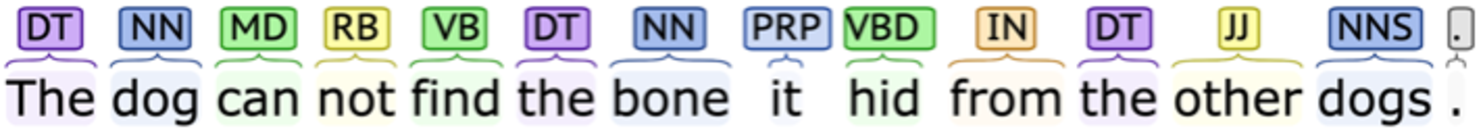
\includegraphics[width=0.95\textwidth]{dog-pos.pdf}
\caption{\label{fig:intro:dog-pos}The structure of POS tags for the
  sentence \emph{\dquoted{The dog cannot find the bone it hid from the
      other dogs.}}~This image shows the tag set used in Penn
  Treebank~\cite{marcus-etal-1994-penn}.}
\end{figure}

\begin{figure}[!tbp]
\centering
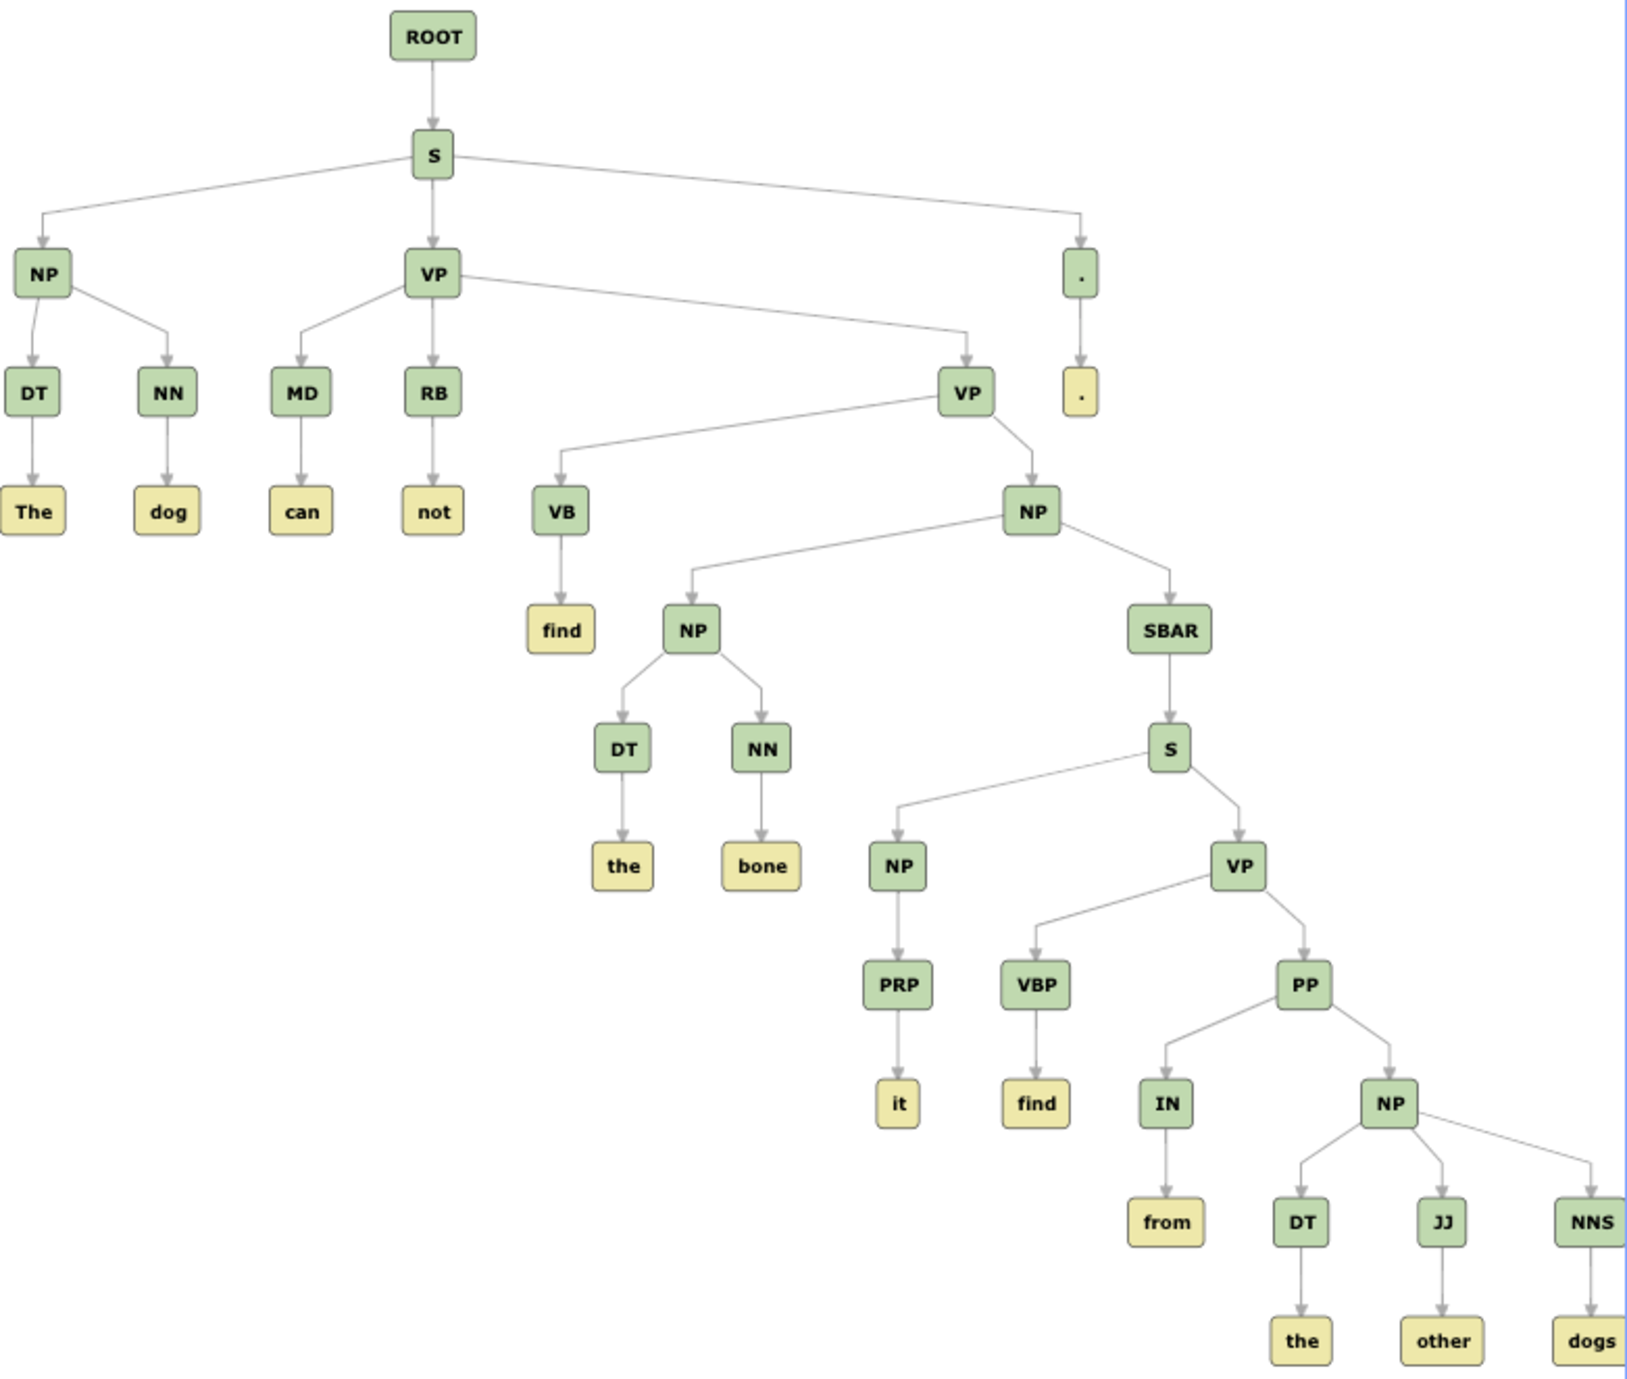
\includegraphics[width=0.95\textwidth]{dog-tree.pdf}
\caption{\label{fig:intro:dog-tree}The structure of constituent tree
  for the sentence~\emph{\dquoted{The dog cannot find the bone it hid
      from the other dogs.}}}
\end{figure}

\begin{figure}[!tbp]
\centering
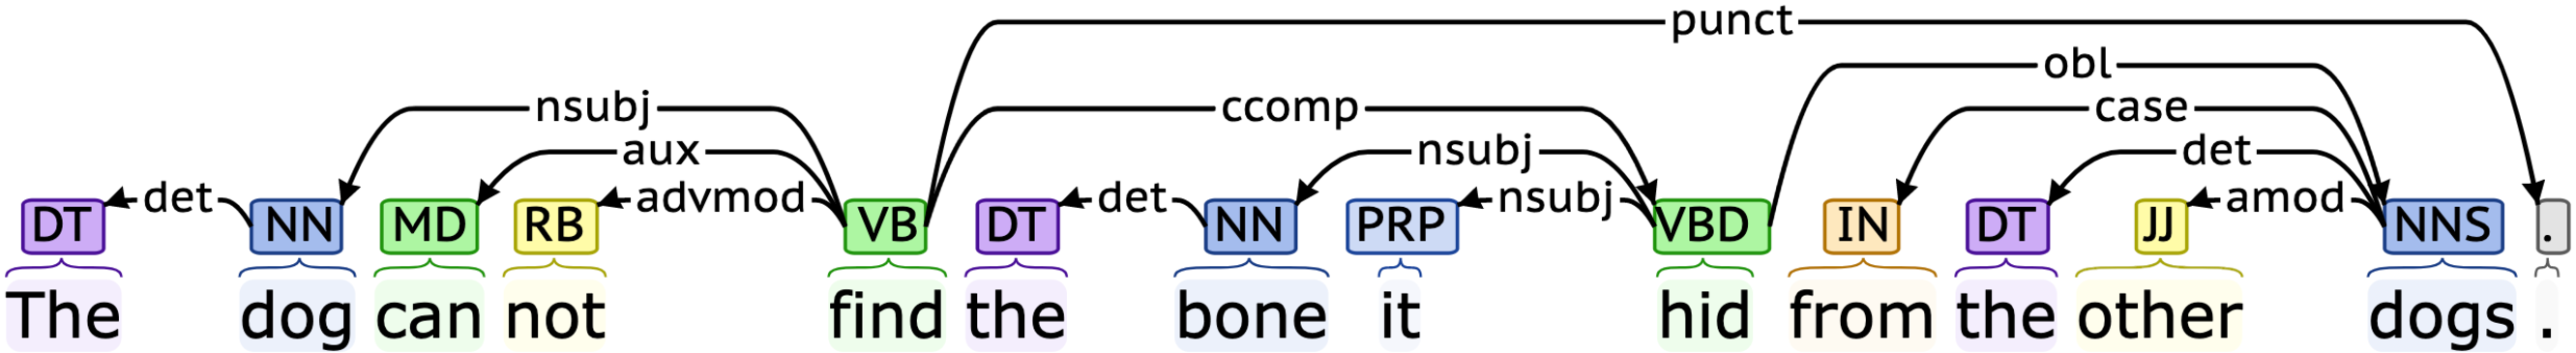
\includegraphics[width=0.98\textwidth]{dog-dep.pdf}
\caption{\label{fig:intro:dog-dep}The structure of dependency tree for
  the sentence \emph{\dquoted{The dog cannot find the bone it hid from the
    other dogs.}}}
\end{figure}

Firstly, we illustrate the \kw{classic linguistic structures}, such as
part-of-speech~(POS), constituency and dependency trees. We consider
the sentence \dquoted{The dog cannot find the bone it hid from the
  other dogs.}~as a running example. As shown
in~\autoref{fig:intro:dog-pos}, the part-of-speech tagging assigns
each word in a sentence a part-of-speech tag, such as \lbl{noun},
\lbl{verb},\lbl{adjective}, \lbl{pronoun}. How to capture the
sequential correlations between consecutive tags is the key modeling
challenge for this task.  \autoref{fig:intro:dog-tree} shows the
\kw{constituent tree} structure of the sentence. The constituent tree
parsing requires recognizing the recursive phrase structure of a
sentence, such as noun, verb, prepositional phrases, and their nesting
in each other. \autoref{fig:intro:dog-dep} shows the \kw{dependency
  tree} structure of the sentence. Unlike the constituency structure,
here the dependency structure of a sentence is described in terms of
the directed bilexical grammatical relations between words. Each
labeled arc represents a directed relation from headwords to their
dependents. Besides the above lexical and syntactic structured
information, as shown in the left part of \autoref{fig:intro:dog-amr},
natural language semantics is also widely studied as structured
representations via tasks such as \kw{ word sense diambiguation},
\kw{semantic role labeling} and~\kw{co-reference resolution} and so
on~\footnote{More details about various semantic phenomena will be
  introduced in~\autoref{ssec:bg:broad-mr}}. Such structured
information is widely used in classical feature-engineering based NLP
system~\citep[\eg,][]{Joh:Nug:08,hovy2010s,punyakanok2008importance},
they are still helpful in deep learning based
systems~\citep{moosavi-strube-2018-using,strubell-etal-2018-linguistically,bowman-etal-2016-fast}.

Secondly, we exmaine \kw{broad-coverage meaning
  representations}. Besides the above structures capturing specific
lexical, syntactic or semantic information, a broad-coverage semantic
representation is a general-purpose meaning representation language
aiming to represent the multiple phenomena in a single structure for
broad-coverage text. \autoref{fig:intro:dog-amr} shows the Abstract
Meaning Representation~\citep[\kw{AMR},][]{Ban:Bon:Cai:13} of the
example sentence. The node in the graph represents abstract
concepts~\footnote{AMR concepts include PropBank framesets, and other
  special dates, spatial entities, etc. More details about AMR will be
  introduced in~\autoref{ssec:bg:broad-mr}}, and the labeled edges
between the nodes represent the relations between those concepts. As
shown in \autoref{fig:intro:dog-tree}, the node \tquoted{find-01} and
\tquoted{hide-01} represents the word sense predefined in the
Propbank~\cite{Kin:Pal:02}; The connected edges \tquoted{:ARG0} and
\tquoted{:ARG1} captures the semantic roles that can be derived from
the semantic role labelling tasks; While the node \tquoted{dog/d1}
means the subjects for the events \tquoted{find-01,}~\tquoted{hide-01,}~and
\tquoted{possible-01} are the same dog, thus capturing the coreference
information. \autoref{fig:intro:dog-ucca} shows the foundational layer
of Universal Conceptual Cognitive
Annotation~\citep[\kw{UCCA},][]{Abe:Rap:13b}, which is a multilayered
framework for semantic representation that aims to accommodate the
semantic distinctions in the sentence and support open-ended
extensions. Different from AMR, this UCCA foundational layer mainly
forms a tree-like structure, which focuses on the argument structures
of verbal, nominal, and adjectival predicates with also the
interrelations between them. Besides the above two broad-coverage
meaning representations, we also studied the DELPH-IN MRS Bilexical
Dependencies~\citep[\kw{DM},][]{ivanova2012did} and Prague Semantic
Dependencies~\citep[\kw{PSD},][]{hajic2012announcing,miyao2014house}. More
details about their captured semantic content and their structure
properties will be introduced comparatively
in~\autoref{ssec:bg:broad-mr}.

\begin{figure}[!tbp]
\centering
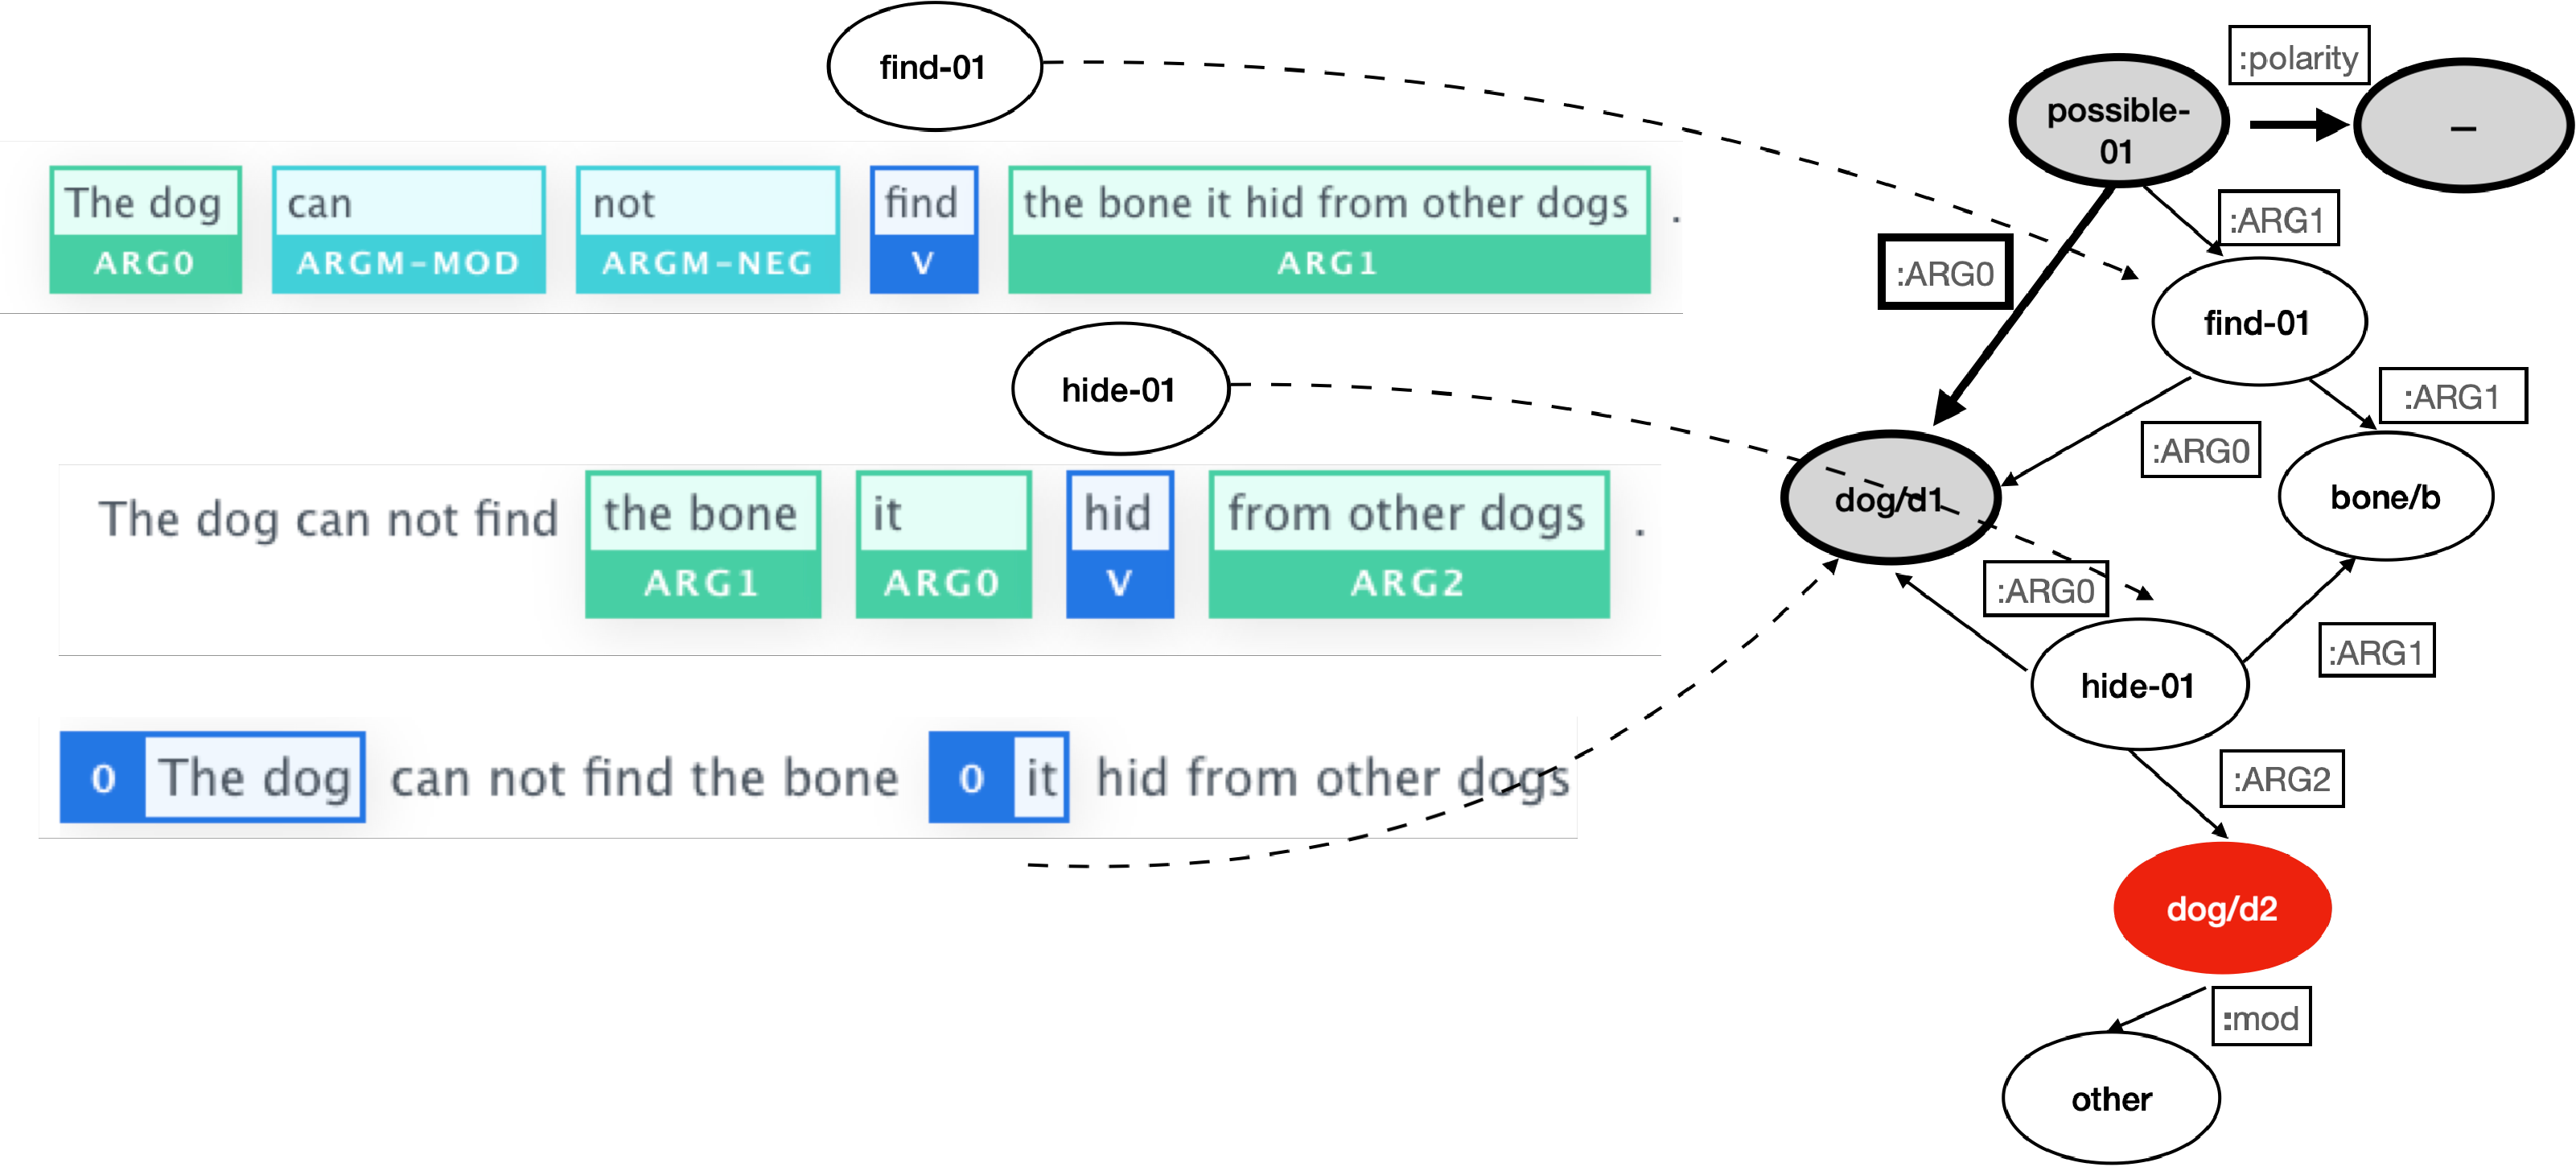
\includegraphics[width=1.0\textwidth]{broad-coverage-mr.pdf}
\caption{\label{fig:intro:dog-amr} The broad coverage meaning
  representation AMR for the sentence \emph{\dquoted{The dog cannot find the
    bone it hid from the other dogs.}} It represents multiple
  phenomena in a single structure, inclduing the predicate-argument
  structure and word sense disambiguiation in semantic role labelling,
  coreference resolution, and so on.}
\end{figure}


\begin{figure}[!tbp]
\centering
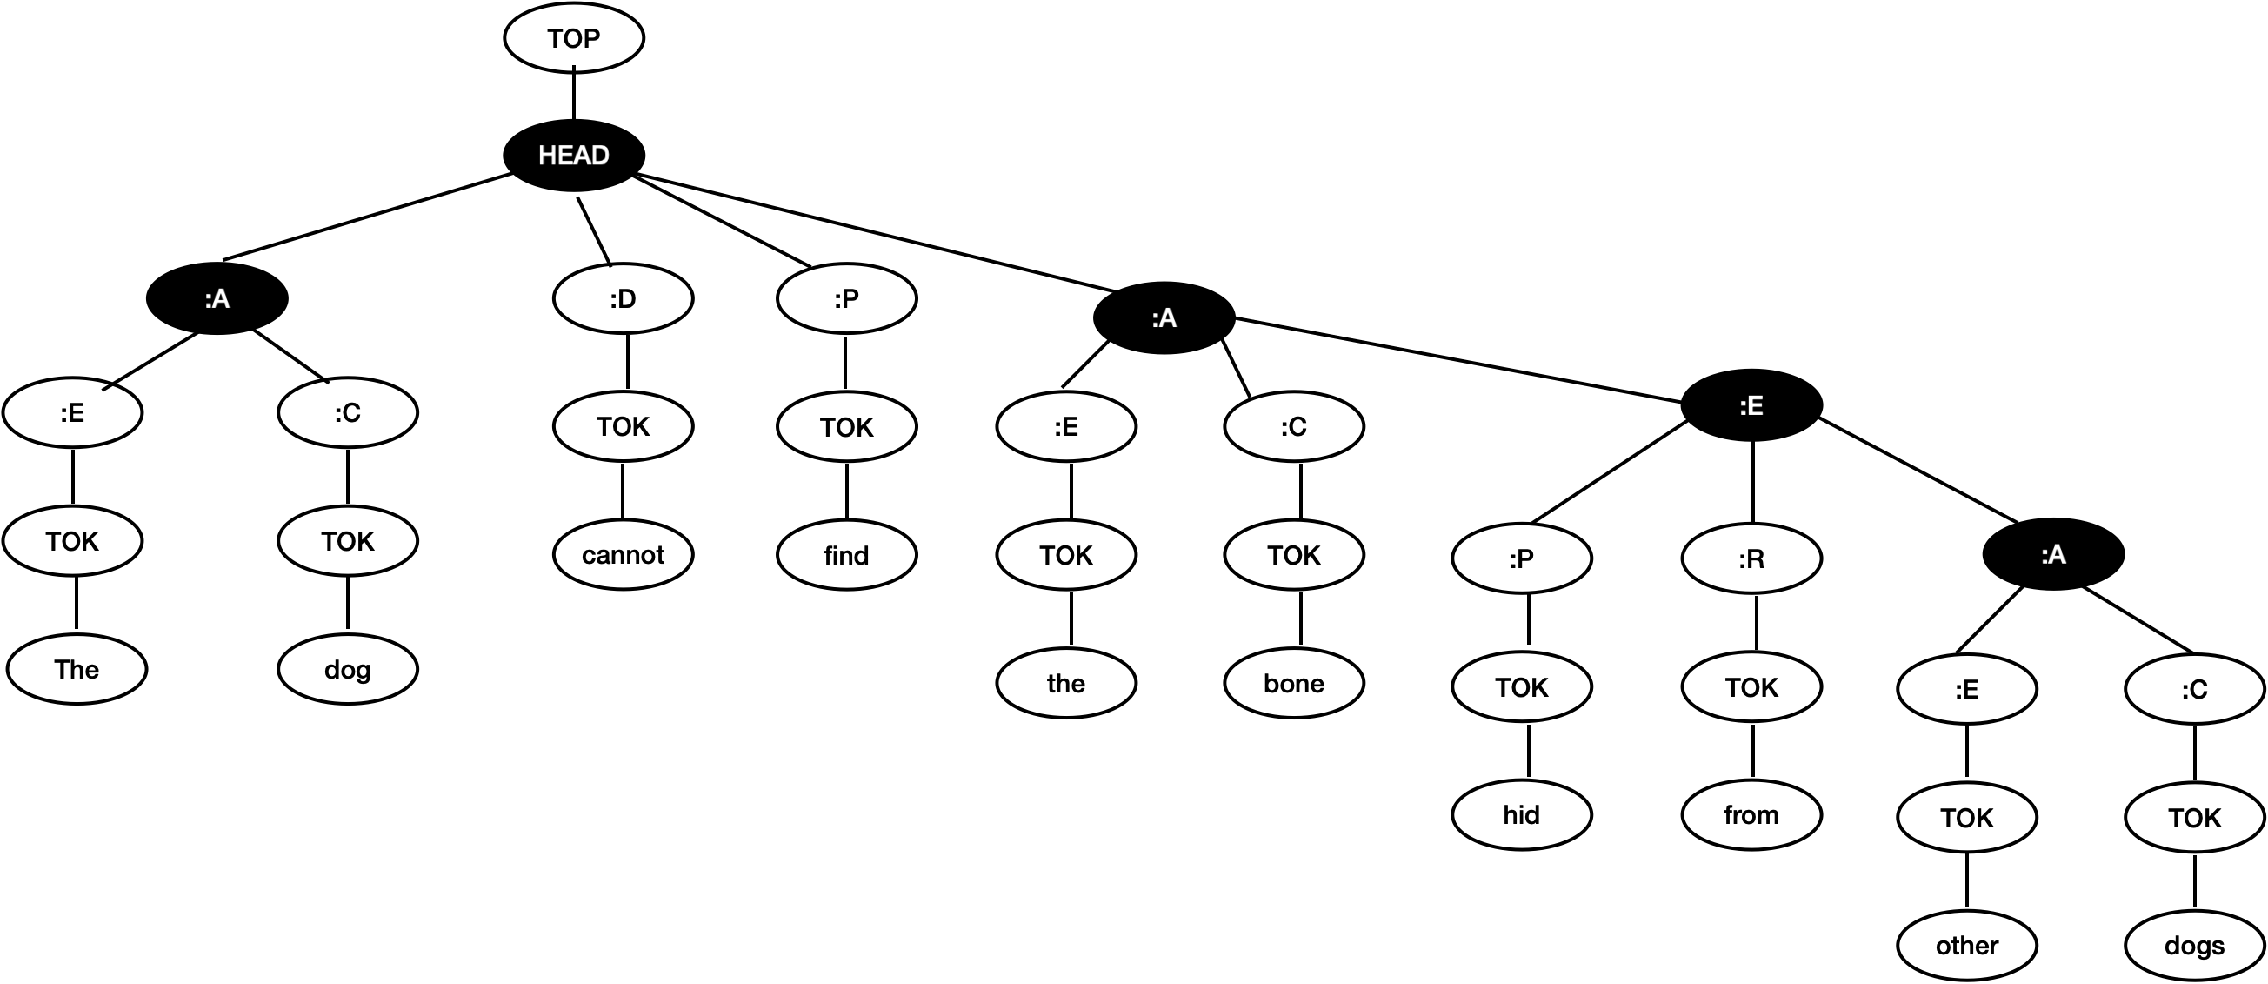
\includegraphics[width=0.90\textwidth]{dog-ucca.pdf}
\caption{\label{fig:intro:dog-ucca} The broad coverage meaning
  representation UCCA for the sentence \emph{\dquoted{The dog cannot
    find the bone it hid from the other dogs.}}}
\end{figure}

Finally, besides the above broad coverage syntactic and semantic
structures in natural language, researchers have designed various
\kw{symbolic representations for specific applications}. Dialogue acts are
firstly designed to represent the speech act or intention of each
utterance, to represent the functions of each utterance in the
dialogue~\citep{wittgenstein2010philosophical,bunt2010towards}. Then
inspired by the case theory~\citep{Fillmore:68}, frame-based
representation in GUS~\citep{bobrow1977gus} are introduced to
represent the state of dialogue, which consists of a collection of
slots and each with a set of possible
values. \autoref{fig:intro:dialogue} shows an example of dialogue
state tracking, where each table is filled with intent, slot, and slot
values, representing a dialogue state for a user turn.

\begin{figure}[!tbp]
\centering
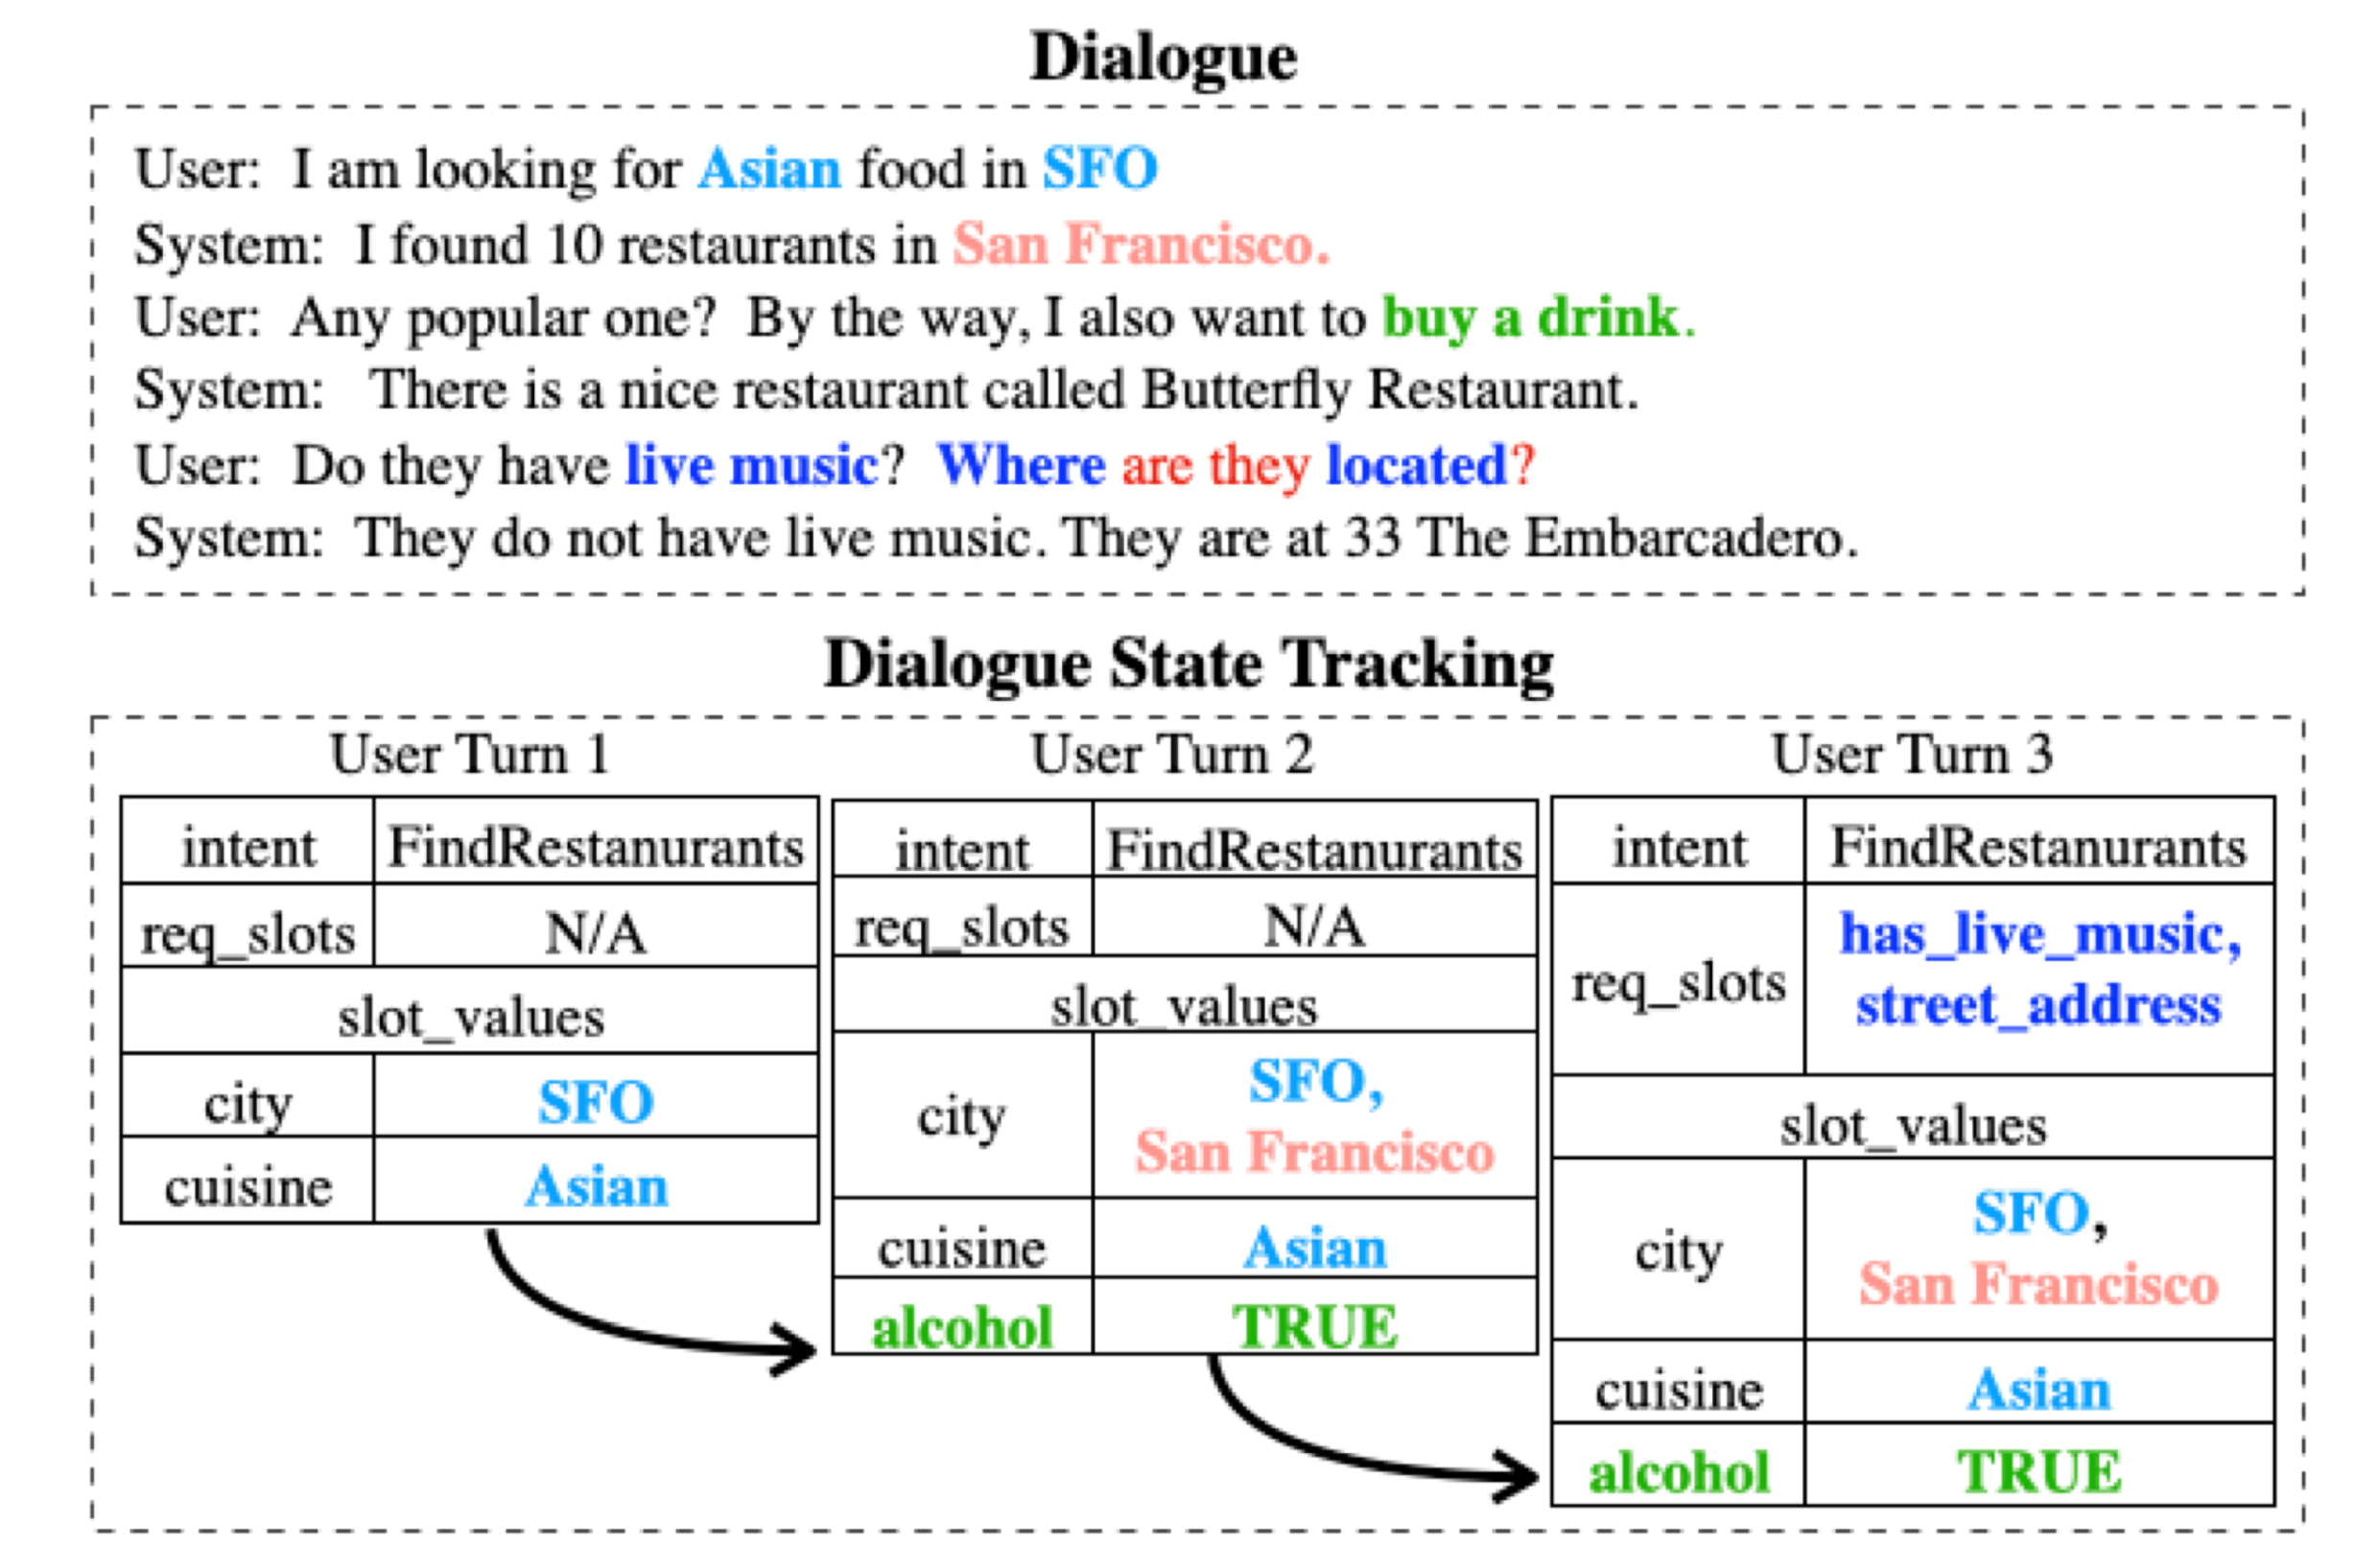
\includegraphics[width=0.98\textwidth]{dialogue-example.pdf}
\caption{\label{fig:intro:dialogue} An example for dialogue state
  tracking.}
\end{figure}

Lexical, syntactic structures, broad coverage semantic representations
and application-specific representations are interpretable to both
human and computers. Such structured representations can enable
rigorous document analysis, easier knowledge organization, and
programmable reasoning. Furthermore, they can be potentially helpful
to offer actionable suggestions to guide human behavior, such as
improving mental health counseling~\citep{tanana2016comparison},
dialogue state tracking~\citep{budzianowski2018multiwoz}, scientific
document analysis~\citep{dernoncourt2017pubmed}, and so on.

With the stunning rise of deep learning, modern NLP systems have
achieved outstanding performance on many benchmark tasks, and offer
helpful services, such as machine translation. Without any prior
knowledge of the syntax or semantic structures for feature
engineering, they feed a large amount of labeled raw data
into an end-to-end deep learning model and outperform many previous
pipeline models built from hand-crafted features. Recently, pretrained
large language models even became the unified base model for many of
the NLP tasks, which further boosts the performance.

However, recent research has shown that such end-to-end NLP systems
often fail catastrophically when given unseen inputs from different
sources or via adversarial attacks. The end-to-end black-box models
lack booth interoperability and robustness, and they are fragile to maintain
when deployed to real users. Using those large language models without
any careful intervention can lead to fairness
issues~\citep{bommasani2021opportunities}.  Using interpretable
symbolic representation in deep learning models can improve both the
efficiency and robustness of NLP systems. For example, combining the
power of neural representation with symbolic AMR representation has
shown great benefits to NLP applications like machine
translation~\citep{song2019semantic},
summarization~\citep{liu2015toward}, question
answering~\citep{kapanipathi2021leveraging} and so on.

Predicting structured representations of text is essential for natural
language processing, even in the deep learning era. In this dissertation, we
ground the studies of natural language structured prediction on both
broad-coverage meaning representations and application-specific
representations. Beyond pure data-driven methods, we primarily study
deep linguistic structured prediction via independent
factorization. We propose two kinds of generic inductive biases to
support the independent factorization for each task, including
structural inductive biases and natural language as inductive biases.

\section{Motivation}
\label{sec:intro:motivation}

In this section, we first examine the need for inductive biases in
machine learning. Then we analyze where current deep learning models
can get inductive biases from, and finally, we highlight some problems
that this thesis addresses inductive biases for deep linguistic
structured prediction.

\subsection{Generalization: The Need for Inductive Bias}
\label{ssec:intro:need-of-bias}

Any system~(natural or artificial) that makes general inferences based on particular and limited data must constrain its hypotheses
somehow. With limited observations and resources~(time, memory,
energy), our human intelligence of generalizing to new environments
makes us efficiently learn when interacting with the world and other
human beings. This efficiency largely depends on many {\bf inductive
  biases} from human intelligence~\citep{Gershman2021WhatMU}, which
can potentially be helpful for machine intelligence. According to
extensive cognitive science
studies~\citep{Spelke1990PrinciplesOO,Bienenstock1996CompositionalityMP,Rehder2003ACT,harlow1949formation,
  Lake2016BuildingMT,Gershman2021WhatMU}, there are many inductive
biases for human intelligence, such as compositionality, causality,
learning to learn, etc. We do not imply machine intelligence
should mimic human intelligence. Instead, we argue that those key
human inductive biases help overcome limited observations and resources
that may inspire us to design machine intelligence.

On the machine intelligence side, the no-free-lunch theorem for
machine learning~\citep{baxter2000model,wolpert1995no} tells us that
inductive biases that influence hypothesis selection is necessary to
obtain generalization. \citet{mitchell1980need} argues that inductive
biases constitute the heart of generalization and, indeed a key basis
for learning itself.

\Paragraph{The Definition of Inductive Bias}
Let us examine a concrete example: the popular supervised learning
setting. We design algorithms that can learn from a set of supervised
training examples to predict a certain target output for an input. The
learning algorithm is presented with some training examples that
demonstrate the intended relationship between the input and output
values. Then the learner is supposed to learn a target function that
captures the correlations between the inputs and outputs. Furthermore,
we hope that the learned target function can approximate the correct
output, even for examples that have not been shown during training. We
call the ability to generalize unseen data a generalization. This
generalization problem cannot be solved without additional assumptions
since unseen situations might have an arbitrary output value. The kind
of necessary assumptions is subsumed in the phrase inductive bias.

%\begin{figure}[!th]
%\centering
%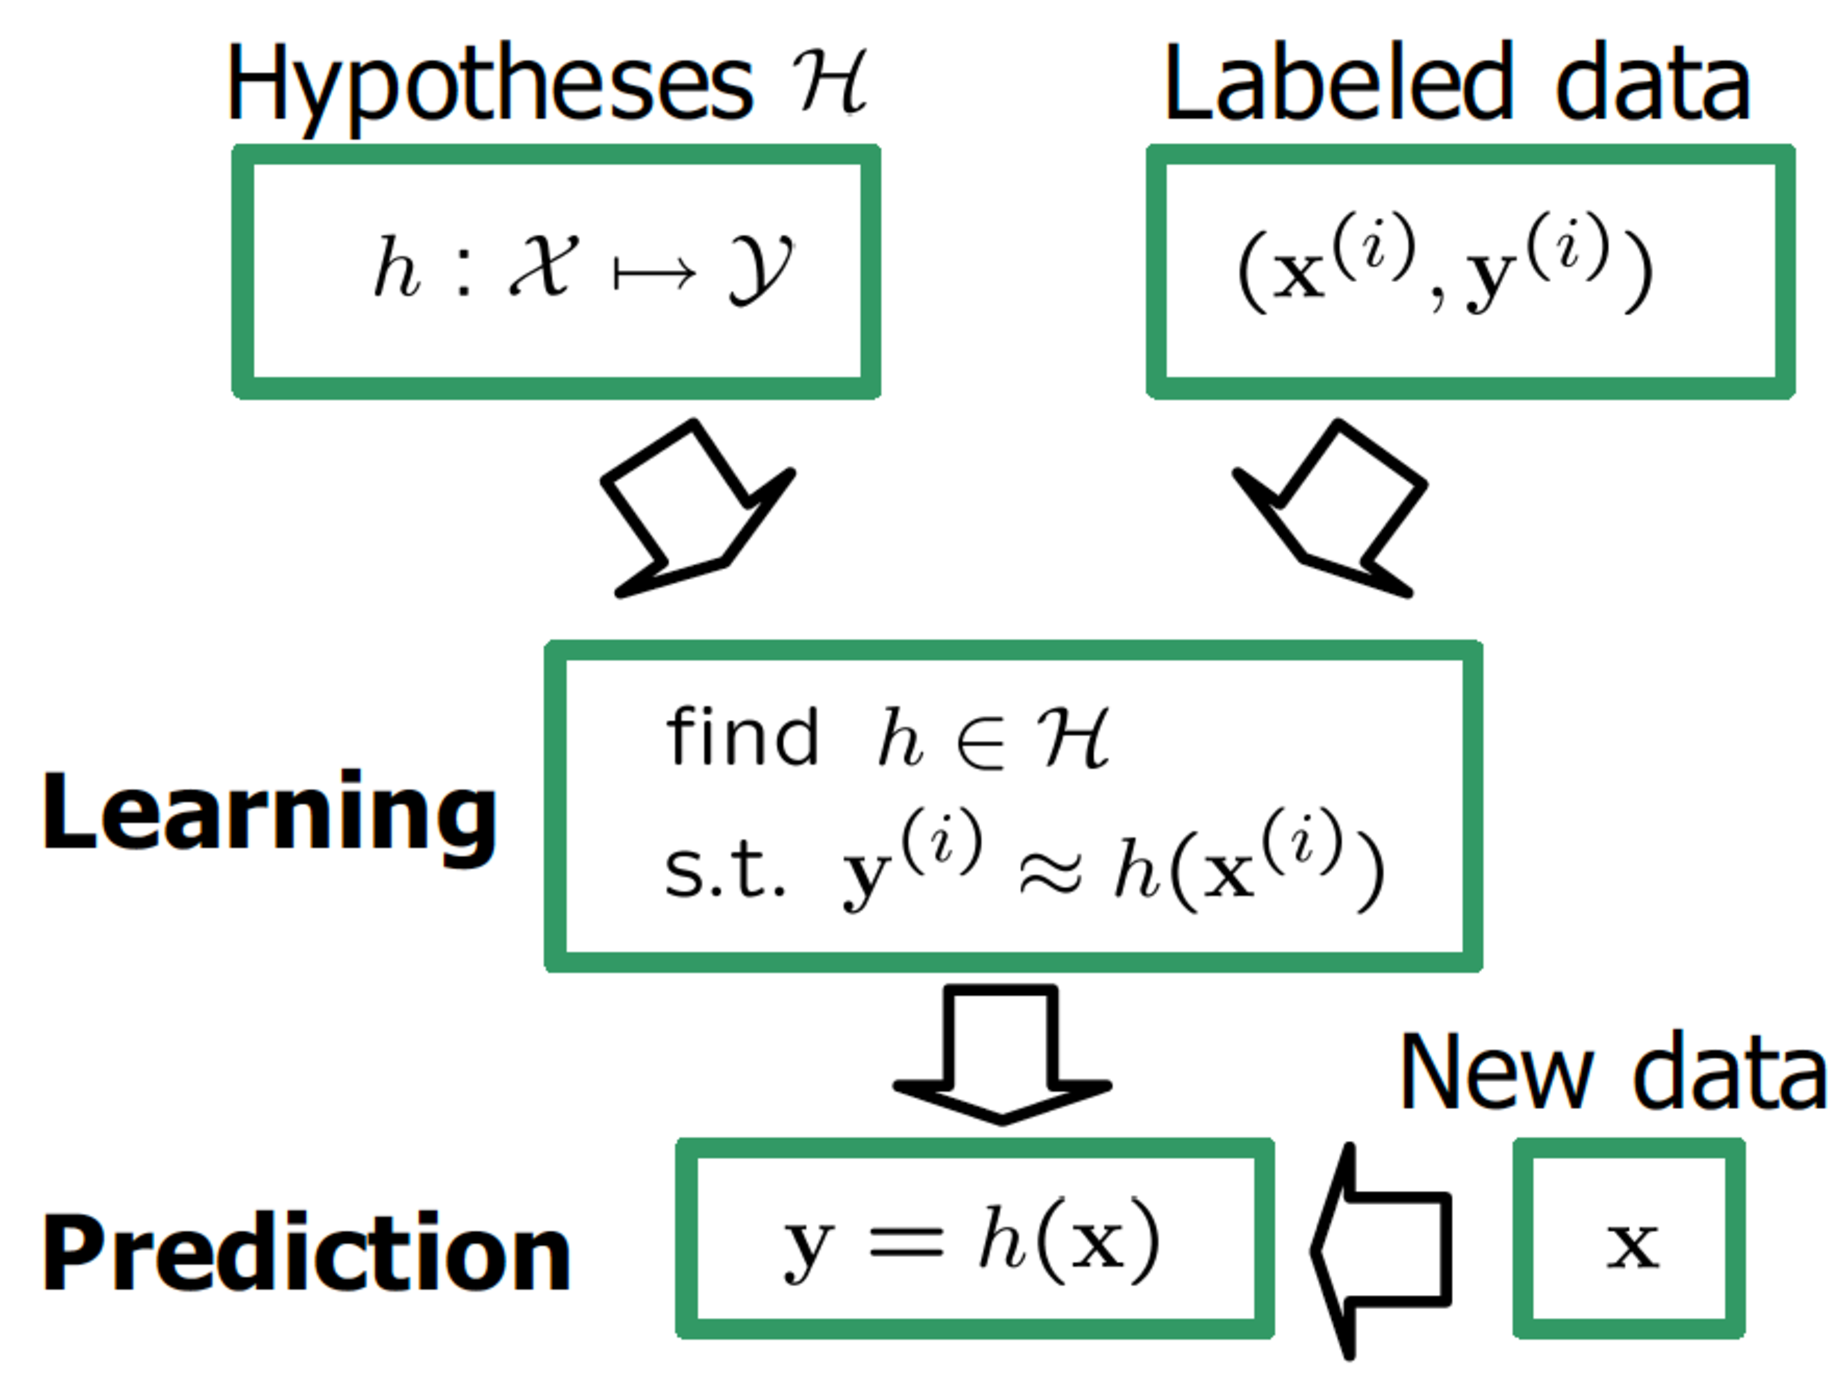
\includegraphics[width=0.80\textwidth]{supervised-learning-hypothesis.pdf}
%\caption{\label{fig:intro-hypothesis}Hypothesis, Generatioalization in
%  Supervised Learning Setting\todo{Current fig is directly copied from
%    Ben Taskar's thesis, redraw it}}
%\end{figure}

In this thesis, following the definition of \kw{bias}
in~\cite{mitchell1980need}, we define \kw{indutive bias} as:

\begin{quote}
  \label{def:bias}
  `Any bias for choosing one generalization over another, other than
  strict consistency with the observed training instances'.
\end{quote}


\Paragraph{The Use of Inductive Biases}
As the definition stated above, inductive biases can be any assumption
beyond the observed training data. In this thesis, we focused on the
supervised learning setting, where observed training data only means
the annotated training data directly available to that task. Inductive
biases are widely studied in the history of machine learning. In the
following, we list common ways of using inductive biases in
machine learning.

For the popular supervised learning setting, let $\mathcal{H}$ refer
to machine learning model families, including deep learning
models. Finding a target hypothesis $h$ is reduced to estimating the
model parameters by fitting the training data. Hence, preferences
beyond training data can naturally be organized into two goals:
choosing the hypothesis class $\mathcal{H}$ and finding the $h$ is
necessary to generalize to new data. For example, different \kw{model
  families} can represent different hypothesis classes. For example,
generalized linear models, such as logistic regression and support
vector machines, can only support linear decision
boundaries. Secondly, inductive biases are also used in \kw{feature
  engineering}. For data that are not linear separable, the choices of
\kw{kernels design} also introduce inductive bias in kernel-based
SVM models. There are also many assumptions about optimization for
finding the specific hypothesis $h$. For example, smoothness
assumptions in the \kw{optimization} method, such as Stochastic
gradient descent, were shown to have better
generalization. \kw{Inference Algorithms}, such as combinatorial
optimization approaches, such as graph cuts, partitions, bipartie
mactching, and dynamic programming can also be involved during the
hypothesis learning, which will also constrain the learning. In this
dissertation, we mainly focus on representation learning. For
inference, we use methods, such as greedy search, maximum spanning
connected graph, and dynamic programming for CKY parsing. Finally, the
biases in the \kw{Training Data} will also influence the hypothesis
finding. It is often the case that available datasets do not exactly
represent the data distribution of interest. One particularly
problematic case is when the dataset is biased against a particular
demographic group, which often leads to model predictions that
unfairly disadvantage members of that group. Hence, \kw{Data
  manipulation} can also help find the desired hypothesis by
augmenting the original training data with inductive biases.

In this thesis, we mainly use \kw{neural architectures} and \kw{data
  manipulation} to support our inductive biases for deep linguistic
structure prediction. To help understand the inductive biases, in
the following, we will first introduce two examples of inductive
biases used in the deep learning era, then we present the main study
the goal of using inductive biases for deep linguistic structured
prediction with independent factorization.

\subsection{Inductive Biases in Deep Learning}
\label{ssec:intro:bias-source}
According to the universal approximation
theorem~\citep{hornik1989multilayer}, a properly parameterized neural
network can represent any function. Furthermore, training data seems
rich enough for many tasks nowadays. It seems purely data-driven deep
learning can learn any target function. Then, what kind of inductive
biases do we need in the deep learning era? In the following, we show two
examples of inductive biases used in computer vision and natural
language processing in the deep learning era.

\begin{figure}[!th]
  \centering
  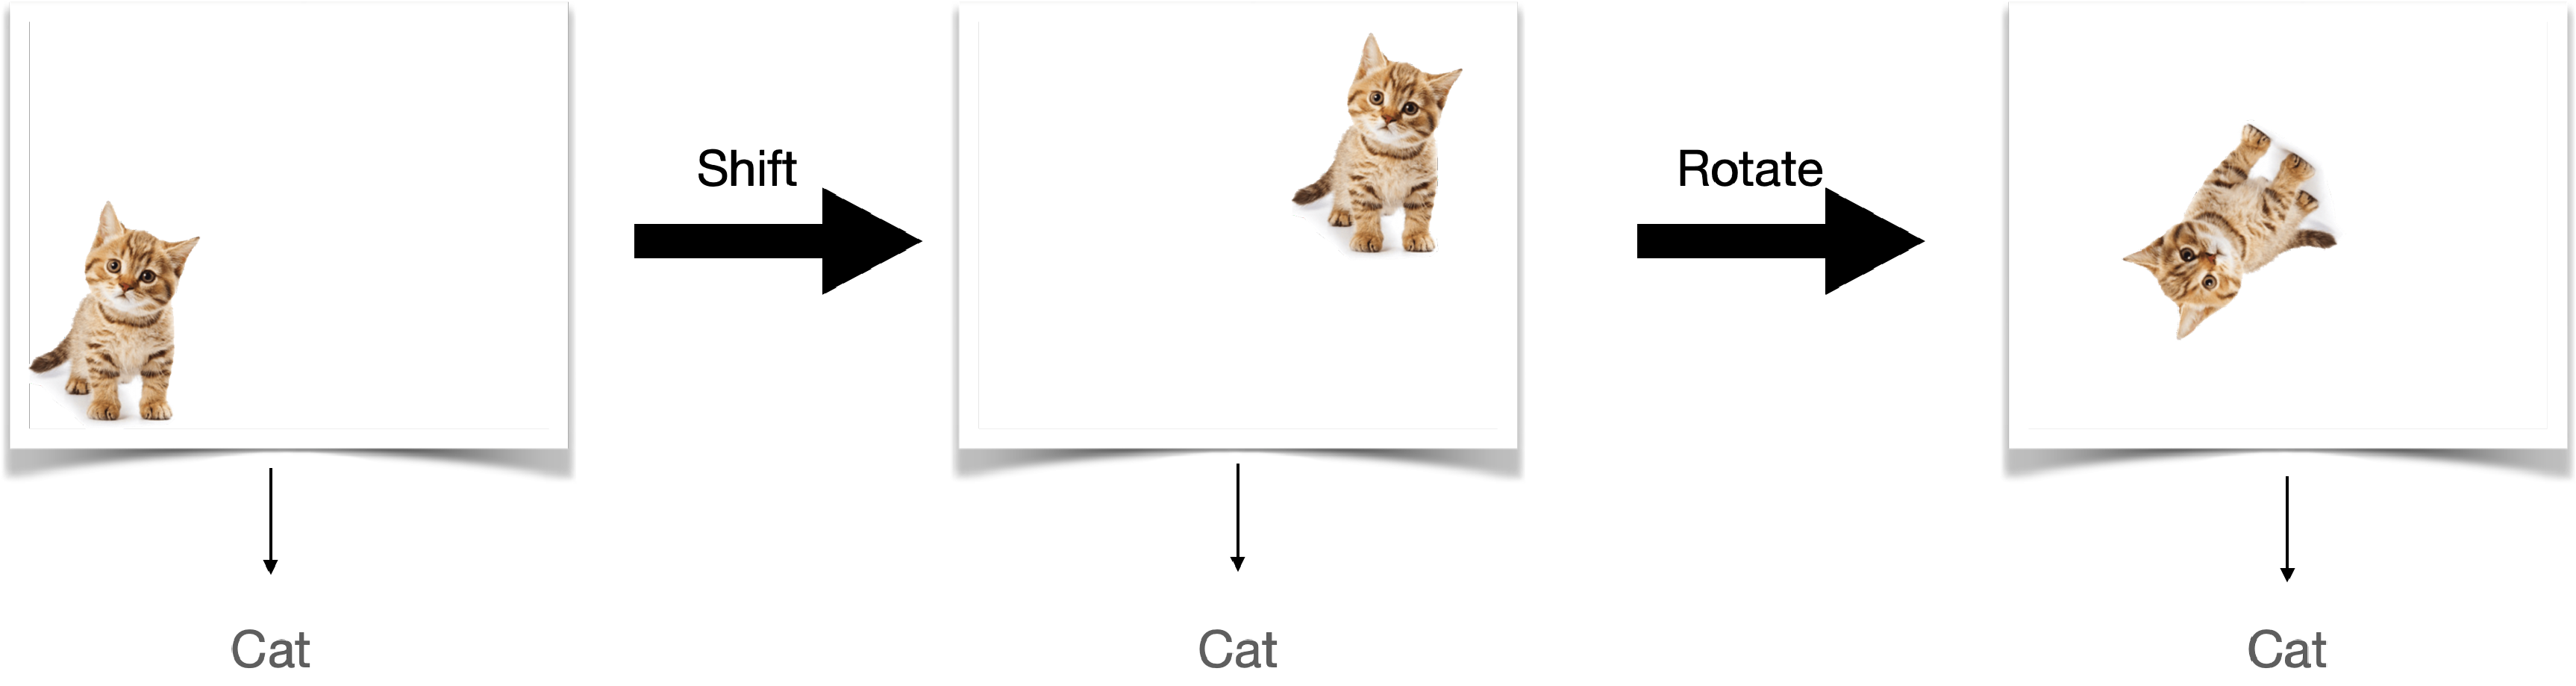
\includegraphics[width=0.98\textwidth]{shift-cat-example.pdf}
  \caption{\label{fig:intro:shift-cat-example}In the image classication
    task, we hope the learned model can still recognize `cat' for the
    unseen image with shifted or rotated cat.}
\end{figure}

\Paragraph{Computer Vision Example: Shift-Invariant in Object
  Classfiction} As the image classification task is shown
in~\autoref{fig:intro:shift-cat-example}, if a model is trained on the
first image with a cat in the bottom-left corner, we hope it can still
predict `cat' when shift the cat to the upper-right corner.
Considering a feed-forward neural network, which can capture any
function, it may fail in this shifted case because not all the
shifts will exist in the training data. Augmenting the training data
with the shifted images may mitigate this problem. However, a more
elegant way is to use convolutional neural networks with a pooling
layer. The pooling operation over convolutional filters is largely
shift-invariant~\citep{zhang2019making}. Beyond the training data, the
inductive bias here assumes the model should be shift-invariant.
Similarly, on the third image
in~\autoref{fig:intro:shift-cat-example}, we also can assume the model
should be rotation-invariant to predict correctly on unseen rotated
cat images~\citep{cheng2016rifd}.

\begin{figure}[!th]
  \centering
  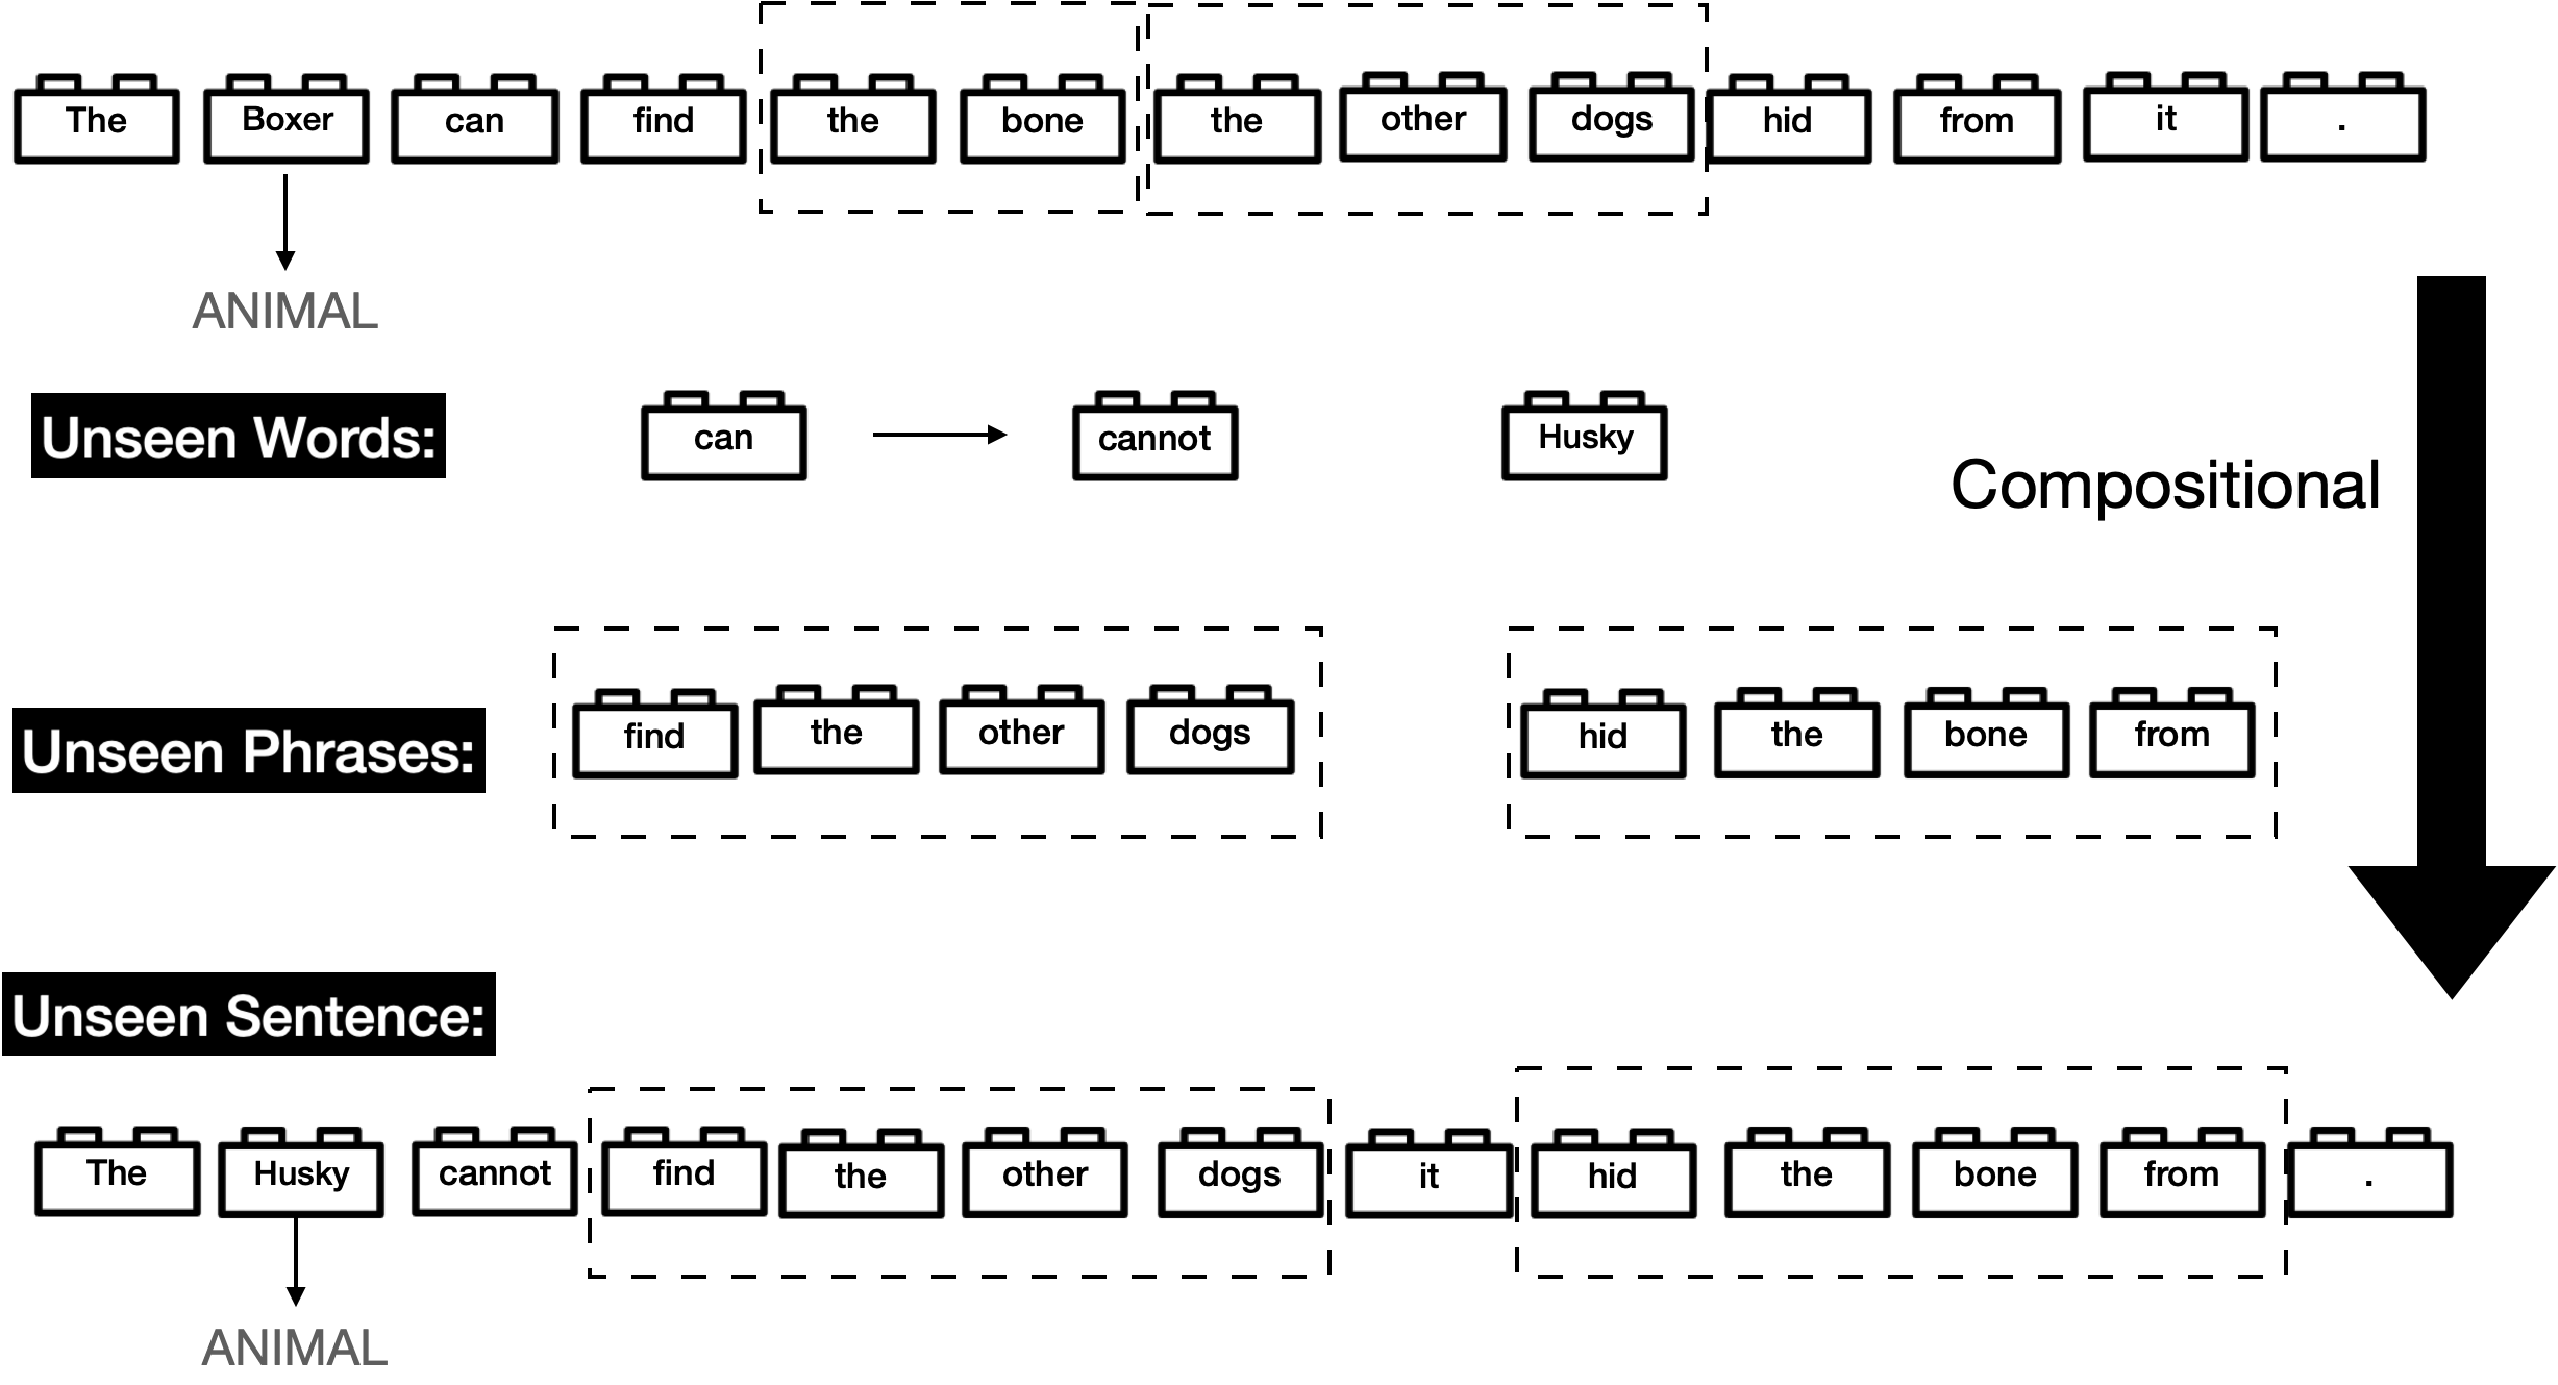
\includegraphics[width=0.98\textwidth]{compositional-dog-example.pdf}
  \caption{\label{fig:intro:compositional-dog-example}In the named entity
    recognization task, we hope the learned model can still recognize
    `dog' for new word 'Husky' in unseen context with newly composed
    words, phases and sentences.}
\end{figure}

\Paragraph{Natural Language Example: Compositionality} For natural
language processing, \autoref{fig:intro:compositional-dog-example} shows
another example of inductive biases in the named entity recognization
task. Natural language is naturally compositional. Beyond the training
data, we mainly make assumptions about the compositional properties
for unseen data. Imagining the training data contains the first
annotated sentence, `The Boxer can find the bone the other dogs hid
from it.', the word `Boxer' is annotated as 'ANIMAL'. Now we add
unseen new words, such as `cannot' and `Husky', and also add unseen
new phrases by swapping the phrases `the bone' and `the other
dogs'. Finally, it forms an unseen new sentence in the bottom of the
figure. Can our model still predict the unseen word 'Husky' in the
unseen sentence as `ANIMAL'? We can augment the training
data by enumerating unseen combinations for the original training
data. However, it is intractable. To achieve this inductive bias about
compositionality, instead of augmenting all combinations, various
techinique are proposed to capture the underlying composing patterns
inspired by linguistic studies. For example, inspired by morphology
study, word piece~\citep{schuster2012japanese} and byte pair
encoding~\citep[BPE,][]{sennrich2016neural} may learn the
representation of unseen words, and they are widely used in the
recent advances in large language models, such as
BERT~\citep{devlin2019bert}, GPT3~\citep{brown2020language}. For
unseen phrases and sentences, inspired by the assumption about
recurrent syntax and grammar, recurrent neural networks~(such as
LSTM~\citep{hochreiter97lstm}, RNN~\citep{mesnil13rnn},
GRU~\citep{chung14gru}, and etc.)  are proposed to capture the
compositional patterns of natural language sequences. Instead of the
the strong recurrent assumption, a weaker word-order assumption also works
quite well by using a positional encoding with self-attention
mechanism in the popular transformer-based
models~\citep{NIPS2017_7181}. Finally, inspired by the distributional
hypothesis, where words that are used and occur in the same contexts
tend to purport similar meanings~\cite{harris1954distributional},
bi-directional architectures are the standard for modeling word
embedding and language models.~(e.g., looking at both the past and future
via Bi-directional LSTM, self-attention, and so on)

Besides the shift-invariant, rotation-invariant and compositional
assumptions for the \kw{input} image and natural language data, there
are other assumptions beyond the training data that can be used in
deep learning era. In this dissertation, we extend the compositional
inductive biases for linguistic structured prediction
tasks.%\todo{SGD generalization,smoothness}
%\todo{Optimization will control the bias shift during learning}


%For example, naturally occurring data will often
%  underrepresent minority groups, so systems can do well on average
%  while having high error rates on these groups
%
% Datasets may also recapitulate stereotypes tied to historical
%%  injustices, which incentivizes models to learn these very
%  stereotypes to achieve the best test accuracy (Zhao et al., 2017,
%  2018; Rudinger et al., 2018). Training data collected from current
%  users of a system will likely be skewed towards users for which the
%  system works well, leading to a feedback loop in which underserved
%  users become increasingly underrepresented in the training data
%  (Hashimoto et al., 2018).
%\todo{Data augmentation for different pertubation}
%\todo{Realistic distribution shift}

\subsection{Independent Factorization for Deep Lingusitic Structured
  Prediction}
\label{ssec:intro:bias-dsp}

For systematic generalization, the search for appropriate inductive
biases is necessary for deep linguistic structured prediction.

First, beyond the compositionality of input natural language, we
believe that both the input text and output structured symbolic
representations will follow the principle of compositionality. The
composition of input natural language and the composition of output
representations are correlated with each other. Hence, we propose to
use the \kw{independent factorization} framework to study the
compositional inductive biases in natural language and its output
structures.

\subsubsection{Independent Factorization}
\label{ssec:intro:ind-factorization}

Let us denote an observation $x \in \mathcal{X}$. It can be any natural
language text, such as the sentence ``The dog cannot find the bone it
hid from the other dogs" or a dialogue segment as shown
in~\autoref{fig:intro:dialogue}. We define an output structured
prediction for $x$ by $y \in \mathcal{Y}(x)$. Here $y$ is a structured
symbolic representation for $x$. For example, $y$ could be a sequence
of part-of-speech tags in~\autoref{fig:intro:dog-pos}, a constituent
tree in~\autoref{fig:intro:dog-tree} or a dependency tree
in~\autoref{fig:intro:dog-dep}. It can also be a broad-coverage
meaning representation, like AMR, UCCA, or a dialogue state table. To
represent the target function $y=f(x)$, we adopt the popular
energy-minimization strategy by defining $f(x)$ as the minimizer of an
auxiliary energy optimization problem.
\begin{equation}
\label{eq:argmin}
f(x) = \argmin_{y \in \mathcal{Y}(x)} E(x, y),
\end{equation}
where $E(x,y)$ is a scoring function representing the energy between
$x$ and a candidate output structure $y$.

In many NLP applications, the candidate output set $\mathcal{Y}(x)$ is
finite but exponentially large, and its size may depend on the input
$x$. For both exact and approximate optimization in
Equation~\ref{eq:argmin}, the main challenges lie on how to model the
representation of \IN~and~\OUT, and the interactions between
them. Practitioners typically employ energy functions with specific
factorization structures to design efficient algorithms, by assuming
the whole energy $E(x, y)$ can be decomposed as a sum of
\textbf{factors} $c$, denoted by $E(x, y) =\sum_{c \in C} E(x, y_{c})$.

A popular choice to represent the factorization is to index both $x$
and $y$ as a set of sub-components $x=(x_{1},..., x_{i},.... x_{N})$
and $y=(y_{1},...y_{j},...y_{M})$. In AMR parsing as shown in
Figure~\ref{fig:intro:dog-amr}, $x_{i}$ can be a word or multi-word
expression in a sentence, while $y_{j}$ can be a single AMR node and
relation.  For dialogue state tracking in
Figure~\ref{fig:intro:dialogue}, $x_{i}$ is an utterance in the
dialog, while $y_{i}$ is the value for each intent and slot in the
predicted frames. A factor $c$ may depend on multiple subcomponents
of $x$ and $y$.

The interdependence assumptions between those sub-components in $x$
and $y$ are key in a structured prediction model. In the
\autoref{chap:background}, we show various representation formalism
~(such as graphical models), structured learning~(max-margin
framework) and inference approaches~(dynamic programming, integer
linear programming) to model interdependence. In this thesis, we
always assume the \kw{independent factorization}, where each factor
$c$ only depends on a well-segmented subset of subcomponents $y_{c}$
and the aligned $x$ components~(anchors)~$x_{c}=a(y_{c})$. In other
words, once the output is decomposed into mutually exclusive output
segments, we consider each segment as an atomic output part, and each
atomic part is independent from the others.

\begin{equation}
    \label{eq:independent-factor}
    \begin{split}
    E(x, y) & =\sum_{c \in C} E(x, y_{c}) = \sum_{c \in C}E(x, a(y_{c}), y_{c})  \\
    \end{split}
\end{equation}

Here, $a(y_{c})$ is the alignment model to find how independent output
parts $y_{c}$ are \kw{anchored} to the constituents of the observation
$x$. Thus the prediction of each $y_{c}$ are independent from each
other, and can be locally decided by its aligned anchors.

Hence, this simple independent factorization can decompose the
structured learning into decomposed local learning~(still constrained
by some global constraints). In this way, independent factorization
largely simplifies the learning of linguistic structured
prediction. More importantly, it also makes the inference tractable,
and thus can be easily employed in the end-to-end neural network
training framework.

Using AMR parsing in \autoref{fig:intro:dog-amr} as an example, the
independent factorization will first segment the output $y$ into small
parts $y_{c} \in seg_{out}(y)$, then find the anchors $x_{c}$ in the
input sentence for each $y_{c}$ from the candidate decomposition set
$seg_{in}(x)$. For example, one of the segmented $y_{c}$ in
Figure~\ref{fig:intro:dog-amr} is a pre-categorized sub-graph
`(possible-01 :polarity -)', and its anchor $a(y_{c})$ is the anchor
word `cannot'. The words `the', 'from' are mapped to empty nodes.
Thus, by leveraging the compositionality of the input and output, and
the alignments between their decompositions, we can focus on the prior
knowledge about the correlations between the input and
output. Futhermore, we can extend that compositionality to help the
model to generalize to unseen inputs and output structures.

\begin{figure}[!th]
\centering
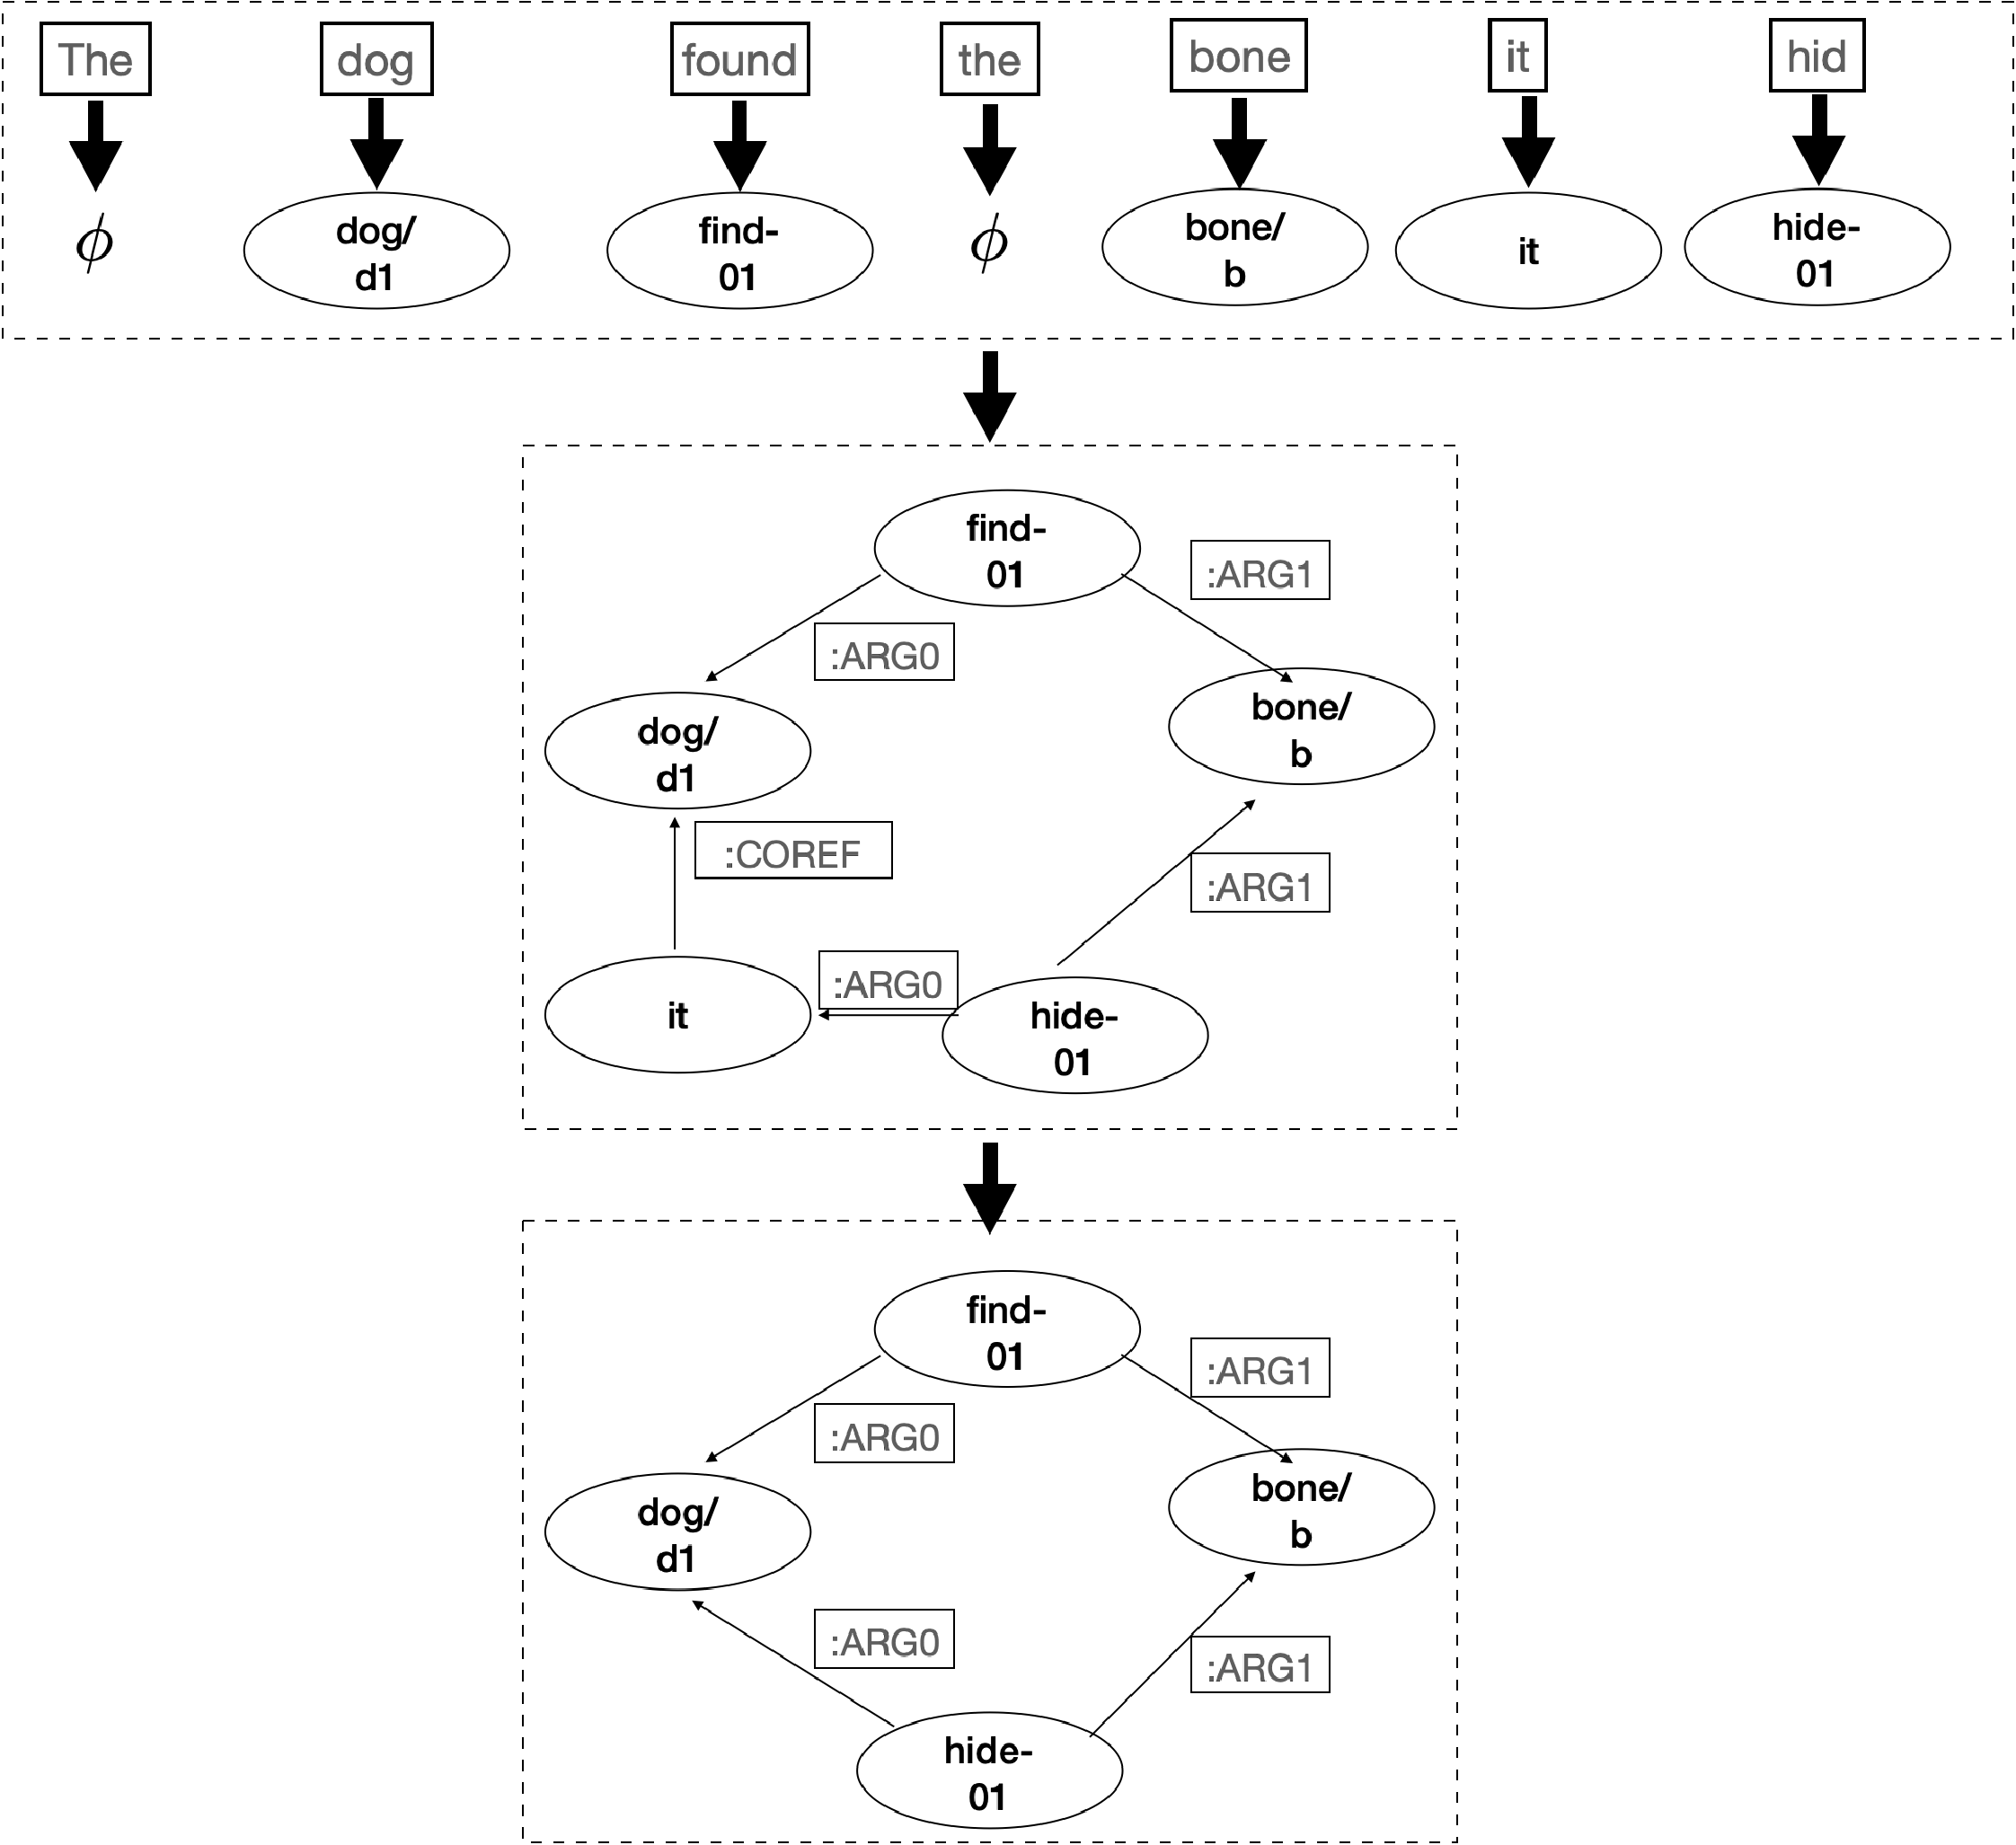
\includegraphics[width=0.80\textwidth]{dog-independent-example.pdf}
\caption{\label{fig:intro:independent-example}Independence
  Factorization for parsing a new sentence "The dog found the bone it
  hid" into an AMR graph}
\end{figure}

During inference, when we encounter a new sentence as shown in
Figure~\ref{fig:intro:independent-example}, we hope the model can
leaverage the seen decomposed mappings in the training data to
generalize to the unseen sentences. In this way, we first prepare a
list of candidate anchors $seg_{in}(x)=\{${`The', `dog', `found',
  `the', `bone', `it', `hide'$\}$, then the model will easily produce
  each independent prediction $y_{c}$ of each anchor as
  $\{\phi,\text{`dog'}, \text{`find-01'}, \phi, \text{`bone'},\text{`it'},
  `hide'\}$ because most of the decomposed inputs are seen in
  previous~\autoref{fig:intro:dog-amr}. Then we assemble the non-empty
  $y_{c}$ by predicting the relations between each other and finally
  forms \OUT~via postprocessing\footnote{The post-processing include
    merging coreference nodes~(as the `dog' and `it'), adding other
    attributes}.

  \Paragraph{Three Steps in Independent Factorizations} In summary, in
  the independence factorization setting, we factorize the input and
  the output via the compositionality of both the input and output,
  and then we hope the model can learn correlations between the
  decomposed input and output parts. Hence, the whole structured
  prediction problem is reduced into three challenges:

\begin{itemize}
\item \textbf{Output Decomposition:} How to decompose the output $y$
  into a set of independent parts $y_{c}$.

\item \textbf{Input Decomposition and Alignment Discovery:} How to decompose $x$ and offer a
  set of candidates that may generate each independent part $y_{c}$.
\item \textbf{Factor Modeling:} How to find the relevant parts
  $x_{a_{y_{c}}}$ in $x$ aligned to ${y_{c}}$ and model the factorized
  energy score $E(x, a(y_{c}), y_{c})$
\end{itemize}

The first question on independently decomposing $y$ is either
straightforward or has been resolved by previously existing methods in
our studied tasks. In this thesis, we mainly focus on the remaining
challenges on modeling alignment and representation learning, which
requires different inductive biases to help with the
modeling. We consider the inductive biases to
help modeling the above structured correlations between the input and
output structures as \textbf{Structual Inductive Biases}, then we also
use \textbf{Natural Language as Inductive Biases} to extend the
independent factorization for cross-domain and cross-task
generalization.

\subsubsection{Structural Inductive Biases}
\label{sssec:intro:structural-biases}
To design the independent factorization for a new task, we require the
prior knowledge about structures of input and output, e.g., proper
input decomposition, or the linguistic analysis on the
semantic-syntactic interface for the alignment information, or more
recent structural bias for deep learning based language modeling.

In this part, using the AMR parsing in
\autoref{fig:intro:structural-bias-example}) as a running example, we
consider the structural inductive biases for its independent
factorization. The first sentence and its corresponding AMR
graph~(left) are in training data, and we need to build a model to
predict the corresponding AMR graph for the unseen sentence. Hence, we
consider the compositionality for both the input and output to offer
more inductive biases beyond the training data. We leave more details
of AMR in \autoref{ssec:bg:amr} and more inductive biases about
decomposing AMR in
\autoref{sssec:lex-phr:lex-output-decomposition}. In this part, we
mainly show the intuitive understanding of the structural inductive
bias for the independent factorization.

\begin{figure}[!th]
  \centering
  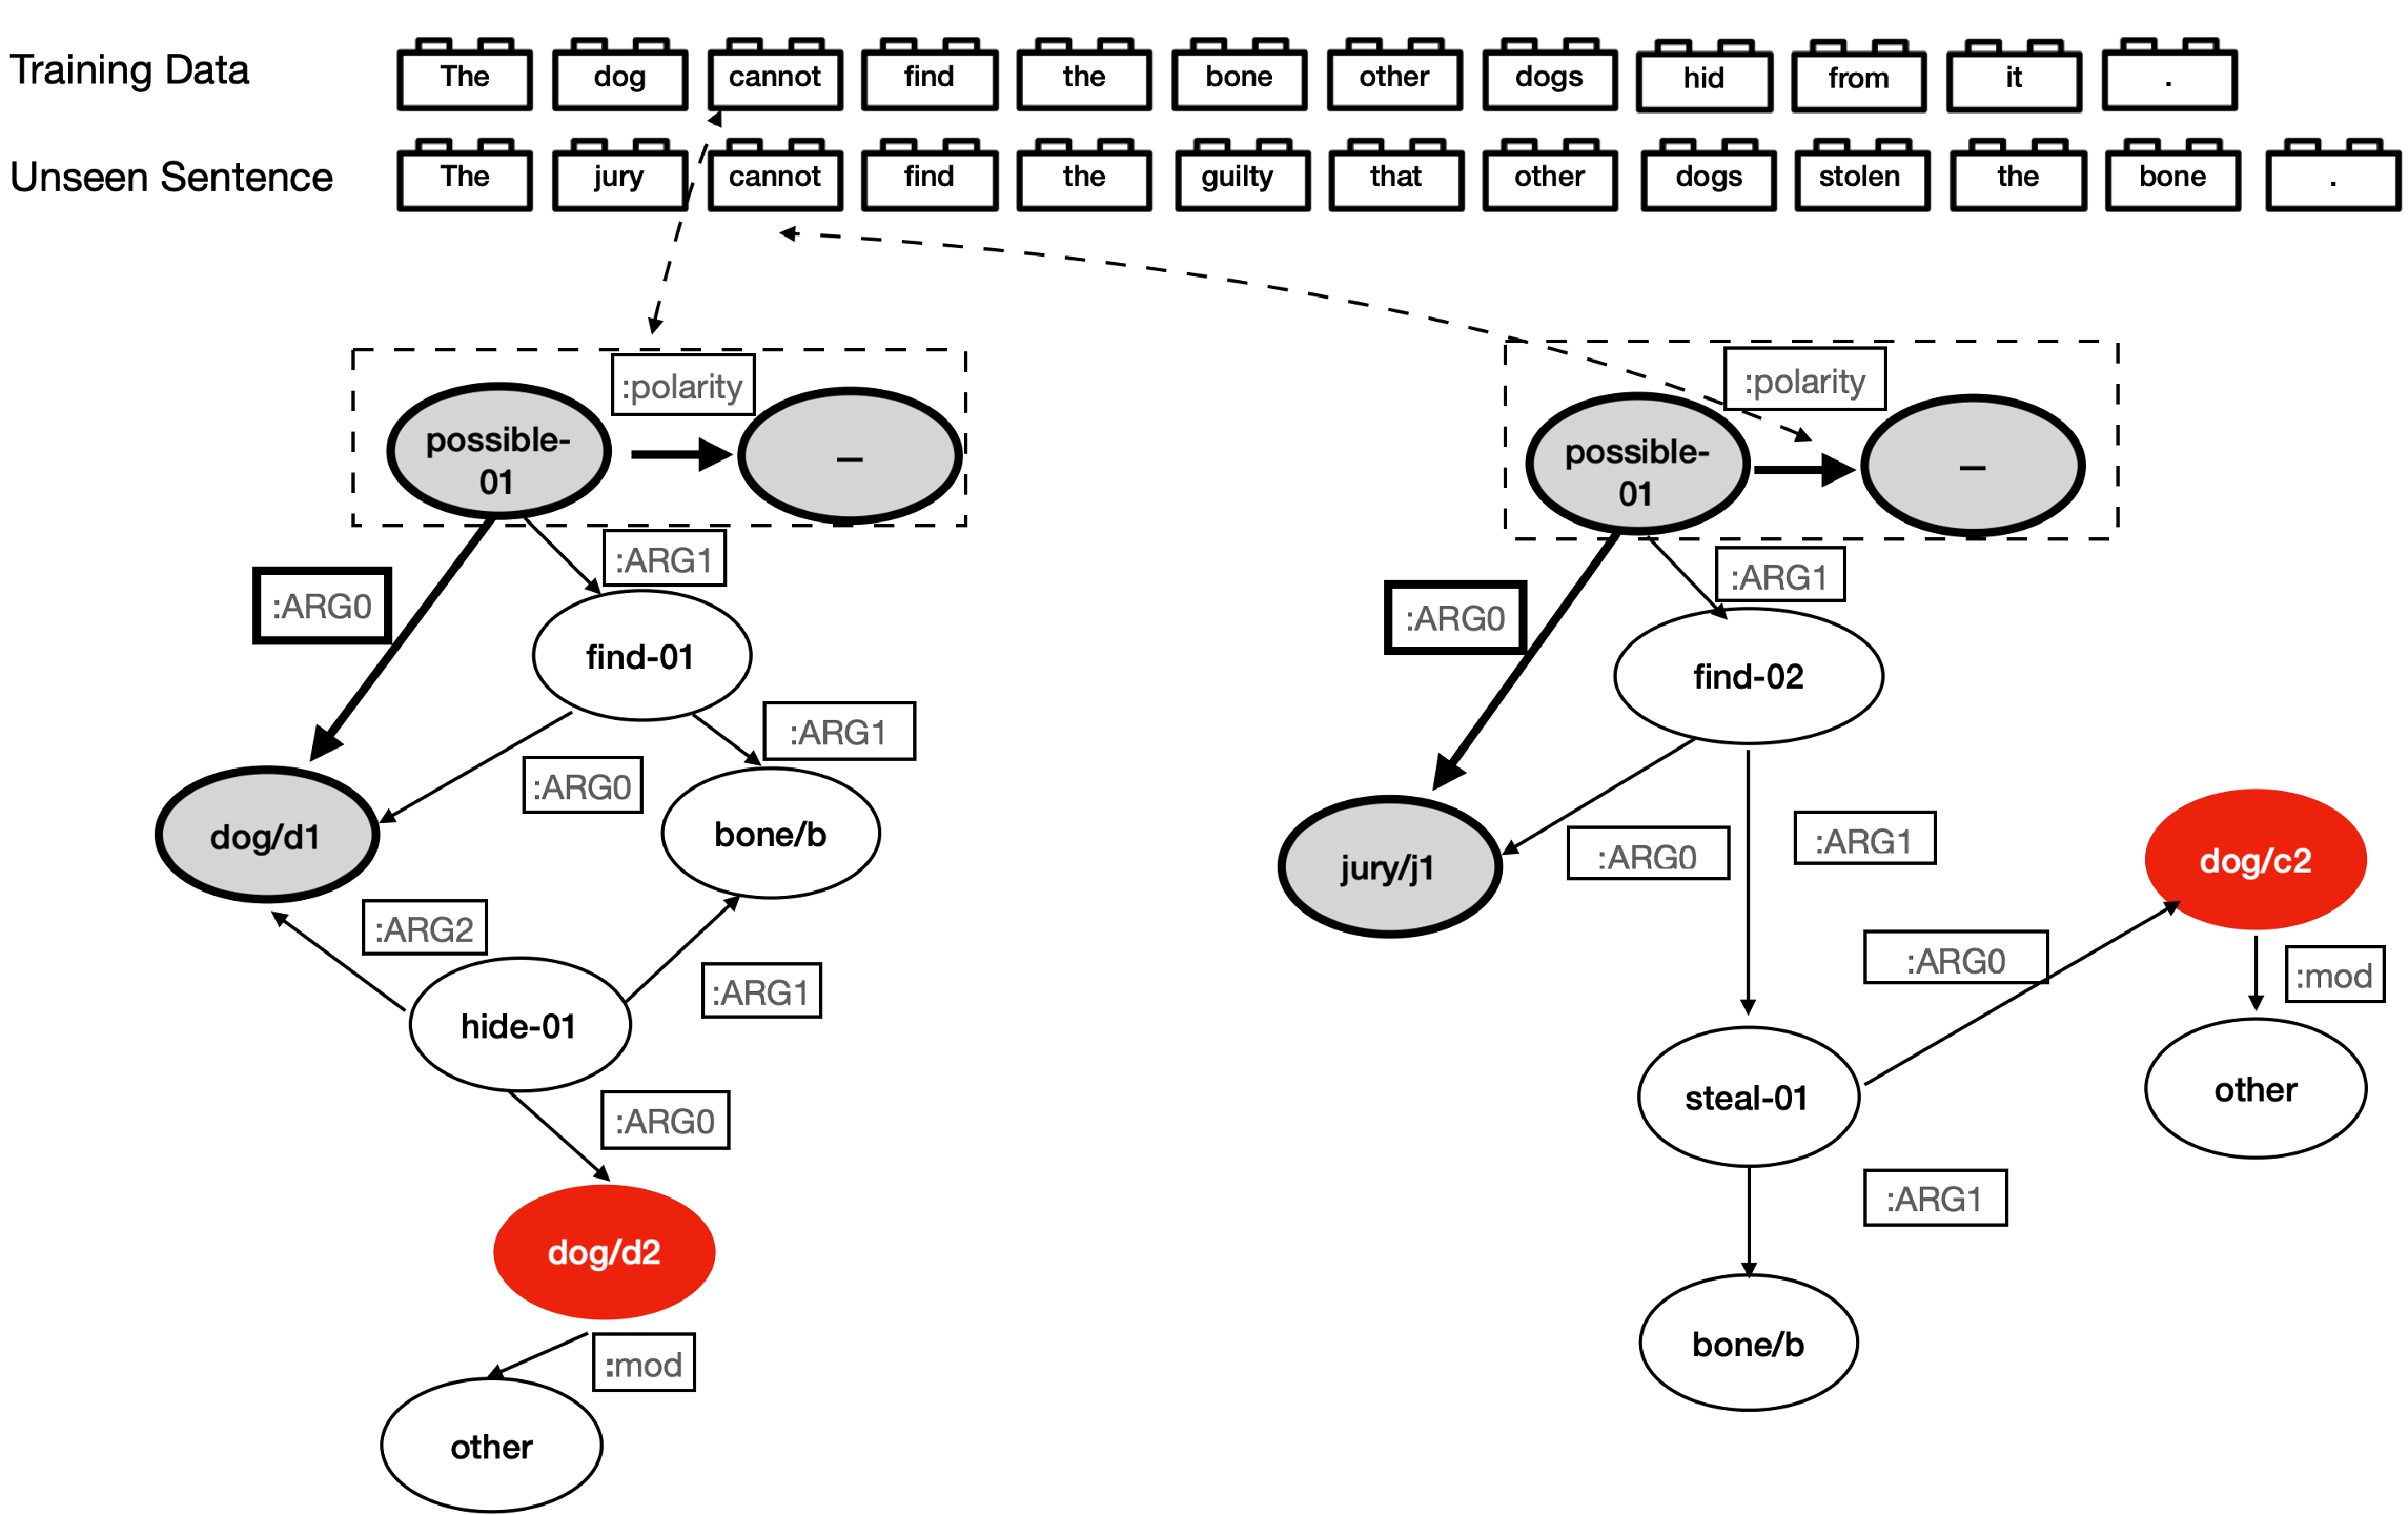
\includegraphics[width=0.95\textwidth]{structural-bias.pdf}
  \caption{\label{fig:intro:structural-bias-example} Structural Inductive
    Biases of AMR decomposition, and AMR alignments.}
\end{figure}

\Paragraph{Output Decomposition} To decompose an AMR graph, we need to
know the meaning of each part of the AMR graph. The nodes in AMR can
be categorized into five main categories~(as shown in
\autoref{fig:intro:structural-bias-example} and a figure in later
section~\autoref{fig:bg:amr}): frame~(e.g., find-01, hide-01), basic
concept~(e.g., dog, jury), string~(``Pierre Vinken"), number (e.g.,
61) and other constant (e.g., `-'), while there many templated
subgraphs used to represent special entities in the AMR, such as
quantities, named entities, special roles, and other entities in
dates, times, percentages, phone, email, URLs. In this part, we mainly
show an example of subgraph segmentation for AMR, which will simplify
the independent factorization. As shown in the left AMR graph, we draw
a rectangle for the subgraph ``(possible-01 :polarity -)", which means
it forms a subgraph when decomposing the output AMR graph. The whole
subgraph will be aligned to the word `cannot' the first
sentence. Furthermore, when there comes the second sentence, for the
same word `cannot' in the new sentence, we hope the model can produce
the same subgraph ``(possible-01 :polarity -)" from it. Besides this
subgraph, other segmented constituents in the left AMR graph will be
each single node. While in other AMR graphs ~(\autoref{fig:bg:amr}),
we must consider the subgraphs used to represent the special
entities. According to the above knowledge about the AMR graph, we use
rule-based recategorization preprocessing to do the segmentation,
which is inspired by the previous work on addressing the data sparsity
issue in AMR
parsing~\citep{Werling:2015up,foland-martin-2017-abstract,Wang:2017vt,Peng:2017ud}

\Paragraph{Input Decomposition and Alignment Discovery} As shown in
the first row of Lego blocks in
\autoref{fig:intro:structural-bias-example}, it naturally forms the
decomposition of the first sentence for the AMR parsing case. However,
for a more complicated case in \autoref{fig:bg:amr}, rather than each
standalone token, we may still need to consider other multiword
expressions and the special entities in the sentence. Furthermore,
when considering the previous UCCA parsing example shown
in~\autoref{fig:intro:dog-ucca}, we also need to decompose the input
sentence into phrases so that it can be easily aligned to the
non-terminal nodes in the decomposed UCCA graph.  Another problem
after the input decomposition is the alignment discovery problem. We
can notice two `dog' lego blocks in the first sentence, and we also
have two `dog' AMR nodes. We have the words `from' in the
sentence. However, it cannot align to any node, the AMR nodes. We need
to build an alignment model to distinguish the alignments between
them. In sum, we must consider the input decomposition with the
inductive biases on the semantic contents in the symbolic
representations and how they are derived from the surface tokens.

\Paragraph{Factor Modeling} The above output and input decomposition
are usually done with prior knowledge about the language and the
corresponding symbolic representations. Once we get the segmented
nodes or subgraphs for output decomposition and the Lego blocks as the
input decomposition, the whole structured prediction problem is
simplified to learning a set of models. For example, we hope the model
can map the words ``cannot" into the subgraph "(possible-01 :polarity
-)", and ``hid" into ``hide-01". When there is explicit alignment
information, it will be easy to model them with aligned input and
output pairs. However, when there are uncertainties about the
alignments, we may need to model the alignment discovery model with
the factor modeling jointly. We propose a latent alignment model for
AMR Parsing in \autoref{sec:lex-phr:graph-based}. Besides that,
considering the same word `find' in both sentences, we need a
discriminative contextualized representation to predict the correct
meaning representation as the `find-01' for the first sentence and the
`find-02' for the second sentence. The efficient contextualized
representation is also the key to making such independent
factorization possible. We will introduce more details of the
two-stage AMR parsing in \autoref{sec:lex-phr:graph-based}, which
introduces how to assemble those local decisions about nodes and edges
into a graph.

In sum, although the independent factorization simplifies structured
prediction into simpler classification problems, however, we need many
inductive biases to make the right design choices. Besides the
above AMR parsing running example, we also design different models with
independent factorization for a set of tasks, e.g., parsing graph-based
representations with
lexical-anchoring~\S\ref{ssec:lex-phr:lex-factorization-analysis} and
phrasal-anchoring~\S\ref{ssec:lex-phr:phr-factorization-analysis},
observing dialog in therapy~\S\ref{sec:snt:task}.

\subsubsection{Natural Language as Inductive Biases}
\label{sssec:intro:language-biases}
We also study natural language description as inductive biases to
describe the function of each decomposed output part. We still take
the AMR Parsing in \autoref{fig:intro:structural-bias-example} as a
running example. When we don't know the meaning of the `find-01' and
`find-02', to make the word `find' in the second sentence can generate
the `find-02' instead of `find-01', it still needs a lot of aligned
pairs about the `find' from other training data to learn. This is true
for both human and machines. However, if we look at the explanation of
``find-01" and ``find-02'' in PropBank~\citep{Kin:Pal:02}, we may
easily find that ``find-01" means discovery, while ``find-02" means
verdict. Hence, human now can easily tell that the second `find'
should predict ``find-02" because it means `verdict" by the jury,
without any more examples about 'find-02". Once we know the
explanation of `find-01' and `find-02', we can disambiguate them
because we understand the meaning of the natural language that is used
for the explanation. We believe that the knowledge in the natural
language can also be used as inductive biases for machine learning. In
this thesis, we mainly extend the independent factorization of
task-oriented dialogue state tracking with natural language
descriptions~\S\ref{chap:sgd}. We show that natural language as
inductive provides great zero-shot performance on unseen dialogue
services.

In sum, motivated by the compositional property of natural language
and related symbolic representation, we propose to use independent
factorization to model the correlations between the input and output
structures. Furthermore, to make the independent factorization work
for our models, we present a detailed analysis of how to do it for
each task, and how to use the above inductive biases to help model the
independent factorization.

%%% Local Variables:
%%% mode: latex
%%% TeX-master: "../../thesis-main.ltx"
%%% End:

%\section{Factorization-Oriented Representation Learning}

\subsection{Modeling Lexicon/Pharsal/Senence-Anchoring}
\subsection{Modeling Symbolic Concepts via Natural Language Description}

%%% Local Variables:
%%% mode: latex
%%% TeX-master: "../thesis-main.ltx"
%%% End:

\section{Contributions}
\label{sec:intro-contri}

\Paragraph{Thesis Statement} Our claim is that by designing
~\kw{Structural Inductive Bias} and \kw{Natural Language as Inductive
  Biases}, models with naive independent factorization can achieve
strong performance at predicting the natural language structures
across multiple broad-coverage meaning representations and
application-specific representations.

\Paragraph{Contributions} In this thesis, focusing on the independent
factorization setting, we show that our proposed indutive biases can
offer discriminative features to achieve competetive and generalizable
performance on broad-coverage meaning representations and
application-specific representations.

We next summarize the main contributions of this thesis, addressing
some of the open problems mentioned in the previous section.

\begin{enumerate}
\item Based on the assumption of independent factorization, we
  proposed a unified parsing framework to support
  both~\textbf{explicit lexical-anchoring} (including DELPH-IN MRS
  Bi-lexical Dependencies~\citep[DM,][]{ivanova2012did} and Prague
  Semantic
  Dependencies~\citep[PSD,][]{hajic2012announcing,miyao2014house}),
  and \textbf{implicit lexical anchoring}~(AMR). Over 16 teams in the
  shared tasks, my parser~\citep{cao2019amazon} \kw{ranked 1st on AMR,
    6th in DM, and 7th in PSD}. By combining Perturb-and-MAP
  sampling~\citep{papandreouperturb} with differentiable
  Gumbel-Softmax Sinkhorn Networks~\citep{mena2018learning}, we can
  approximately infer the discrete latent-alignment variable in
  lexical-anchoring of the independent factorization setting. The
  \textbf{phrasal-anchoring} Universal Conceptual Cognitive
  Annotation~\citep[UCCA,][]{abend2013universal} and Task-oriented
  Dialog Parsing~\citep[TOP,][]{gupta-etal-2018-semantic-parsing} are
  similar to constituency tree structure, except for unseen phenomena
  such as remote edges and discontinuous spans, we extend the existing
  algorithmic inductive bias for tree structure prediction and
  Cost-augmented CKY inferece to the new UCCA and TOP parsing
  tasks. Powered by strong span-representation learning method, my
  system~\citep{cao2019amazon} \kw{ranked 5/16 on UCCA parsing}, and
  it can be reused for TOP parsing after a few preprocessing steps,
  and outperform serveral baseline models.

\item To provide real-time guidance to therapists with a dialogue
  observer, we decompose the dialog structure analysis with two
  independent prediction tasks: (1) categorizing therapist and client
  MI behavioral codes and, (2) forcasting codes for upcoming
  utterances to help guide the conversation and potentially alert the
  therapist. For both tasks, I studied a hierarchical gated recurrent
  unit (\HGRU) with the \kw{word-level attention} and
  \kw{sentence-level attention} to distinguish different importance of
  words and sentences~\citep{jie2019psycdialacl}. Our experiments
  demonstrate that our models can outperform several baselines for
  both tasks.  We also report the results of a careful analysis that
  reveals the impact of the various network design tradeoffs for
  modeling therapy dialogue.

\item By decomposing the dialogue state tracking into four independent
  sub-tasks, we use natural language description as inductive biases
  to describe the functions of each independent intent/slot labels,
  thus capturing the function overlapping between different
  services. We show that such natural language descriptions can
  support the zero-shot learning for each independent subtask for
  unseen service. We are among the first to use large pretrained
  language models for description-based dialog state tracking. We
  offer detailed comparative studies on how to transfer inductive
  biases to new domains and APIs with overlapping functions and task
  structures, including encoding strategies, supplementary
  pretraining, homogenuous and heterogeneous evalutions.
\end{enumerate}


%%% Local Variables:
%%% mode: latex
%%% TeX-master: "../../thesis-main.ltx"
%%% End:


\section{Thesis Outline}
\label{sec:intro:roadmap}
To coherently present the thesis, we think it is helpful to discuss
prior work related to an application in its own chapter, instead of
putting them all in a single chapter. Therefore, we include a section
of related work at the end of each application chapter. This thesis is
divided into five parts, which we described below.

\Paragraph{Chapter 2. Background} The first part systematizes the
background of this theis study in two sections:
\begin{itemize}
\item \kw{Structures in NLP.} We first provide the necessary
  background about structures in natural languages for better exposing
  our contributions in remaining chapters.
\item \kw{Structured Prediction, Learning and Inference.} We summerize
  the recent advances in deep structured prediction with respect to
  representational formaliam, learning and inference
  respectively. Epsecially, we overview the development of
  representation learning methods for natural language, from feature
  selection to deep learning based representation learning methods.
\end{itemize}

\Paragraph{Chapter 3. Structural Inductive Biases for Lexical and
  Phrasal Anchoring} In this chapter, we provide lexical and phrasal
anchoring analysis to decompose the output structures into locally
dependent parts, where each part can be derived from its anchoring
words or phrasal in the input sentence. For lexical-anchoring, we
propose a unified model to support both explicit and implicit
alignment information between each input parts and output parts. For
phrasal-anchoring, we compared different ways to learn the
contextualized representation to rerepsent the span, and how they can
bring discriminative features to our locally-dependent model. We show
that with the above lexical and phrasal-anchoring based structural
inductive biases for energey factorization and contextualized
representation learning, our model can learn efficient discriminative
features for the anchor representations and still achieve high
performance in the locally-dependent model.

\Paragraph{Chapter 4. Structural Inductive Biases for Sentence and
  Dialog} In the following two chapters, we extend our study to
structures beyond a single sentence. In this chapter, We study the
seuquential dialog flow structure in a style of therapy called
Motivational
Interviewing~\cite[MI,][]{miller2003motivational,miller2012motivational},
which is widely used for treating addiction-related problems.
Sentence-level tags called Motivational Interview Skill Codes are
designed to represent the intention of each utterance and the dialogue
flow of the whole therapy session. By developing a modular family of
neural networks categorizing and forcasting the dialog flow in the
form of MISC codes, we show that the above mechanisms on dialogue
representation can efficiently model the sequential structure of
dialogue flow.

\Paragraph{Chapter 5. Natural Language as Inductive Biases} In this
chapter, we study using natural language descriptions to represent the
meaning of output symbols~(Intents and Slots) in task-oriented dialog
state tracking, which helps to reduce the poor scalability to transfer
to unseen domain and services. We study three main challenges of using
natural language for label representation: schema encoding,
supplementary training, and description styles.


\Paragraph{Chapter 6. Conclusion and Future Work} This chapter
concludes, by providing a summary of contributions and drawing
possible directions of future work.


%%% Local Variables:
%%% mode: latex
%%% TeX-master: "../../thesis-main.ltx"
%%% End:


%%% Index phrases should be attached to an important word of a phrase,
%%% and are usually best kept on a separate line by terminating the
%%% previous line with a percent comment without intervening space, as
%%% in this example:
%%%
%%%     \newcommand {\X} [1] {#1\index{#1}}
%%%
%%%     African ungulates,%
%%%     \index{African ungulate}
%%%     like the \X{gnu}, \X{impala}, \X{kudu}, and \X{springbok}
%%%     live mostly in hot climate and consume vegetation.
%%%
%%% However, for this document, we only want lots of index entries to
%%% populate a sample topic index.
\index{Inductive Bias}
\index{Structured Prediction}
\index{Linguistic Structured Prediction}
\index{AMR, Abstract Meaning Representations}
\index{PSD, Prague Semantic Dependencies}
\index{DM, DELPH-IN MRS Bilexical Dependencies}


%%% Local Variables:
%%% mode: latex
%%% TeX-master: "../dissertation-main.ltx"
%%% End:
